%%%%%%%%%%%%%%%%%%%%%%%%%%%%%%%%%%%%%%%%%%%%%%%%%%%%%%%%%%%%%%%%%%%%%%%%%%%%%%%%%%
% TEMPLATE INFORMATION:
%%%%%%%%%%%%%%%%%%%%%%%%%%%%%%%%%%%%%%%%%%%%%%%%%%%%%%%%%%%%%%%%%%%%%%%%%%%%%%%%%%
% Stylish Article LaTeX Template - Version 2.1 (1/10/15)
% Downloaded from: http://www.LaTeXTemplates.com
% License: CC BY-NC-SA 3.0 (http://creativecommons.org/licenses/by-nc-sa/3.0/)

%%%%%%%%%%%%%%%%%%%%%%%%%%%%%%%%%%%%%%%%%%%%%%%%%%%%%%%%%%%%%%%%%%%%%%%%%%%%%%%%%%
% TEMPLATE AUTHORS:
%%%%%%%%%%%%%%%%%%%%%%%%%%%%%%%%%%%%%%%%%%%%%%%%%%%%%%%%%%%%%%%%%%%%%%%%%%%%%%%%%%
% ORIGINAL AUTHOR: Mathias Legrand (legrand.mathias@gmail.com) 
% EXTENSIVE MODIFICATIONS: Vel (vel@latextemplates.com)
% FURTHER MODIFICATIONS: Saleem Ameen (saleem.ameen@live.com)
%%%%%%%%%%%%%%%%%%%%%%%%%%%%%%%%%%%%%%%%%%%%%%%%%%%%%%%%%%%%%%%%%%%%%%%%%%%%%%%%%%

%---------------------------------------------------------------------------------
%	PACKAGES AND DOCUMENT CONFIGURATION
%---------------------------------------------------------------------------------

\documentclass[fleqn,10pt]{Stylesheet} % Document font size and equations flushed left
\usepackage[english]{babel} % Specify a different language here - english by default
\usepackage{lipsum} % Required to insert dummy text. To be removed otherwise
\usepackage{subcaption}
\usepackage{gensymb}
\usepackage{array}
\newcolumntype{L}{>{\arraybackslash}m{12cm}}

%---------------------------------------------------------------------------------
%	COLUMNS
%---------------------------------------------------------------------------------

\setlength{\columnsep}{0.55cm} % Distance between the two columns of text
\setlength{\fboxrule}{0.75pt} % Width of the border around the abstract

%---------------------------------------------------------------------------------
%	COLORS
%---------------------------------------------------------------------------------
\definecolor{color1}{RGB}{139,0,2} % Color of the article title and sections
\definecolor{color2}{RGB}{0,20,20} % Color of the boxes behind the abstract and headings
\definecolor{color3}{RGB}{189,141,29} % Color of the golden lines

%---------------------------------------------------------------------------------
%	HYPERLINKS
%---------------------------------------------------------------------------------

\usepackage{hyperref} % Required for hyperlinks
\hypersetup{hidelinks,colorlinks,breaklinks=true,urlcolor=color2,citecolor=color1,linkcolor=color1,bookmarksopen=false,pdftitle={Title},pdfauthor={Author}}

%---------------------------------------------------------------------------------
%	ARTICLE INFORMATION (E.G. JOURNAL, AUTHORS)
%---------------------------------------------------------------------------------

\JournalInfo{Mars Society, 2020} % Journal information
\Archive{Mars City State Design Competition} % Additional notes
\PaperTitle{Korolev Crater Special Administrative Region} % Article title
\Authors{Alex Sharp\textsuperscript{1}*, Epi Pereria\textsuperscript{2}} % Authors
\affiliation{\textsuperscript{1}\textit{OrionVM}} % Author 1 affiliation
\affiliation{\textsuperscript{2}\textit{Artist}} % Author 2 affiliation
\affiliation{*\textbf{Corresponding author}: alex@asharp.id.au} % Corresponding author
\Keywords{} % Keywords: Keyword1 --- Keyword2 --- Keyword3
\newcommand{\keywordname}{Keywords} % Defines the keywords heading name

\graphicspath{ {figures/} }

%---------------------------------------------------------------------------------
%	ABSTRACT
%---------------------------------------------------------------------------------
\Abstract{\lipsum[1]~}

%---------------------------------------------------------------------------------
%  START DOCUMENT
%---------------------------------------------------------------------------------

\begin{document}
\flushbottom % Makes all text pages the same height
\maketitle % Print the title and abstract box
\thispagestyle{empty} % Removes page numbering from the first page

%---------------------------------------------------------------------------------
%	INTRODUCTION
%---------------------------------------------------------------------------------

\section*{Introduction}
%\addcontentsline{toc}{section}{Introduction} % Add to Table of Contents
In this paper, we seek to outline the central processes and systems that would underpin a successful colony on Mars. To provide a substantive analysis, we limit ourselves to dealing most with the processes that we think are most unique to the Martian environment that cannot simply be transplanted directly from modern societies on Earth as well as those that are unique to our proposed colony on Mars, the Korolev Crater Special Administrative Region. 

The Korolev Crater Special Administrative Region (‘KCSAR’) is a special administrative region of the United States of America established in the 2060s. It is located within the Korolev Crater, an ancient ice-covered impact crater at 73 degrees North, 163 degrees East on Mars. The Crater was selected because it contains around 2000 $km^{3}$ of water ice, which provides an abundant supply of water and serves as a simple and cheaply implemented cold sink and radiation shield. KCSAR is a subglacial city, housed within interconnected domes constructed into the ice, as seen in figure \ref{fig:dome}, and small domes that sit atop it to offer a means of egress to the Martian surface. It extends in a crescent shape from the northernmost point of the crater along its inner rim.

% TODO: Maybe we should make a comment introducing the idea of "this is what it will be at first" and "this is where it will eventually be" referencing the terraform

% TODO: IF we have space, setting out the scene for the structure of this paper

\begin{figure}
    \centering
    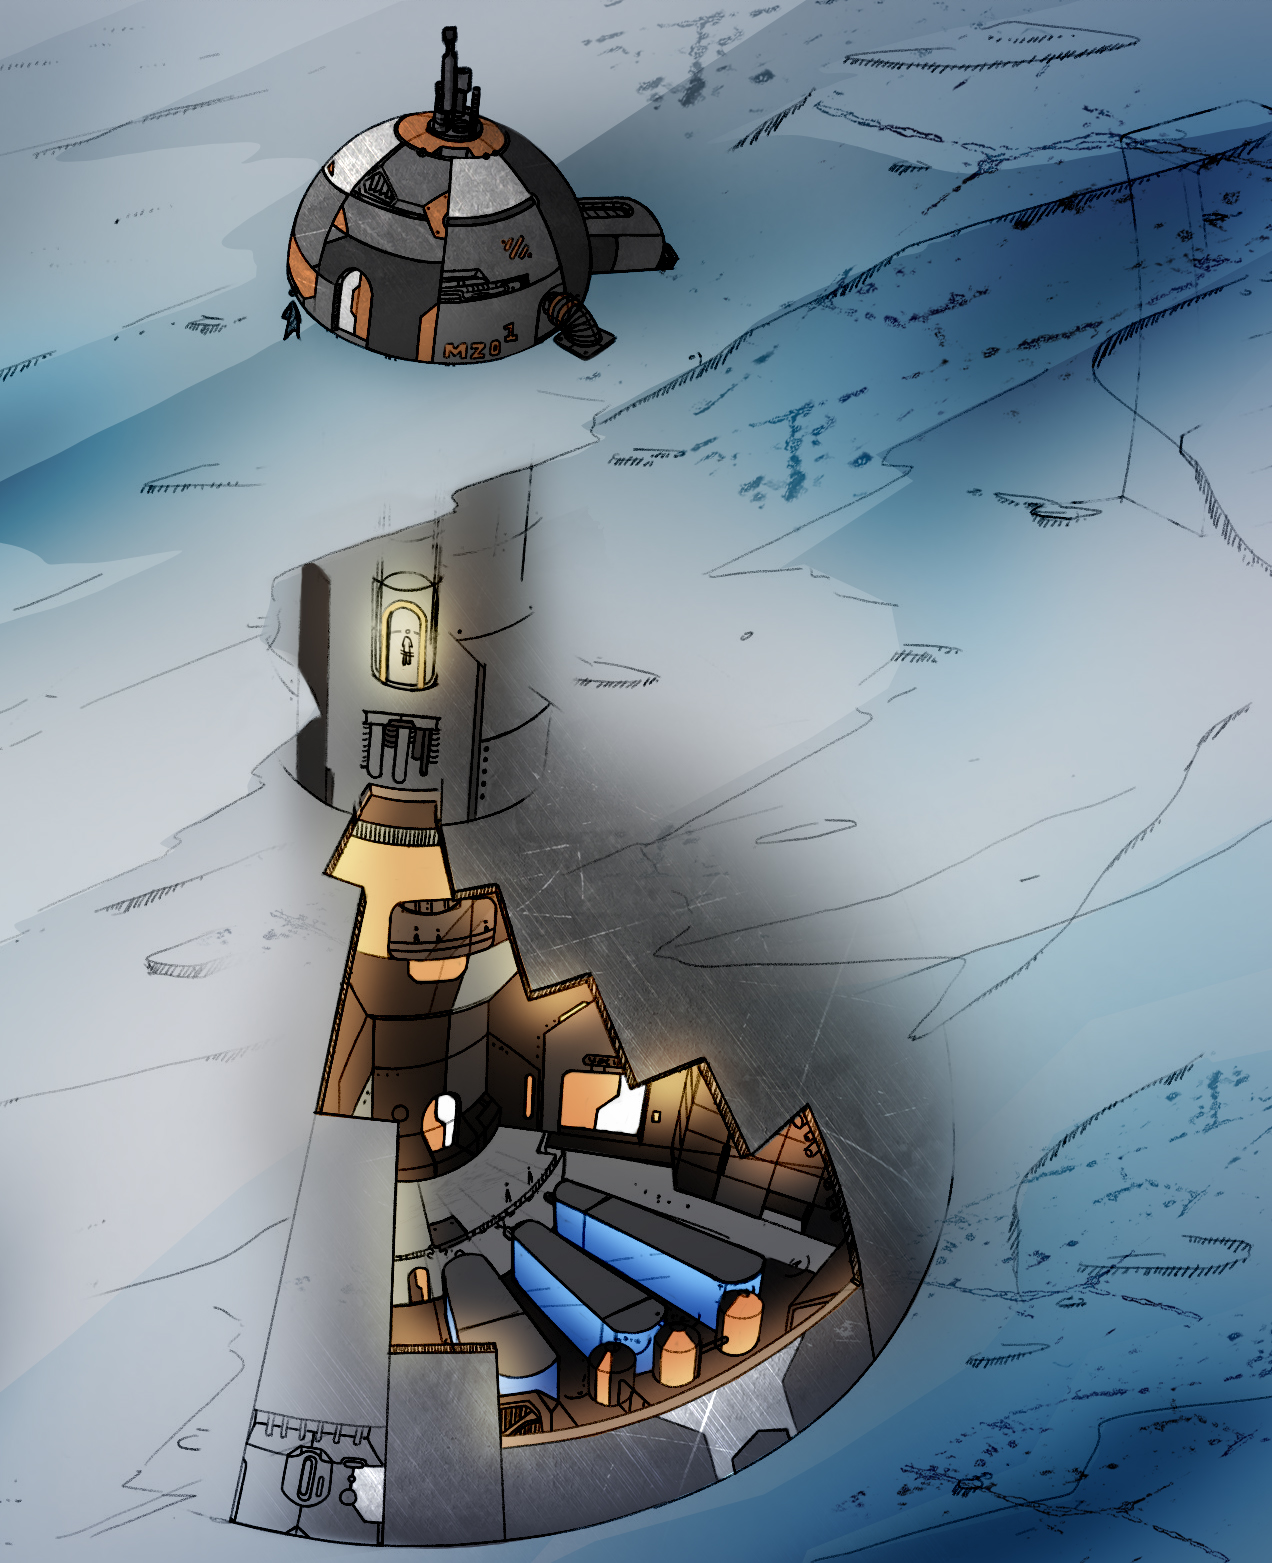
\includegraphics[width=\linewidth]{art/dome_crop.jpg}
    \caption{Artist's rendition of the dome under the ice.}
    \label{fig:dome}
\end{figure}

\begin{figure}
    \centering
    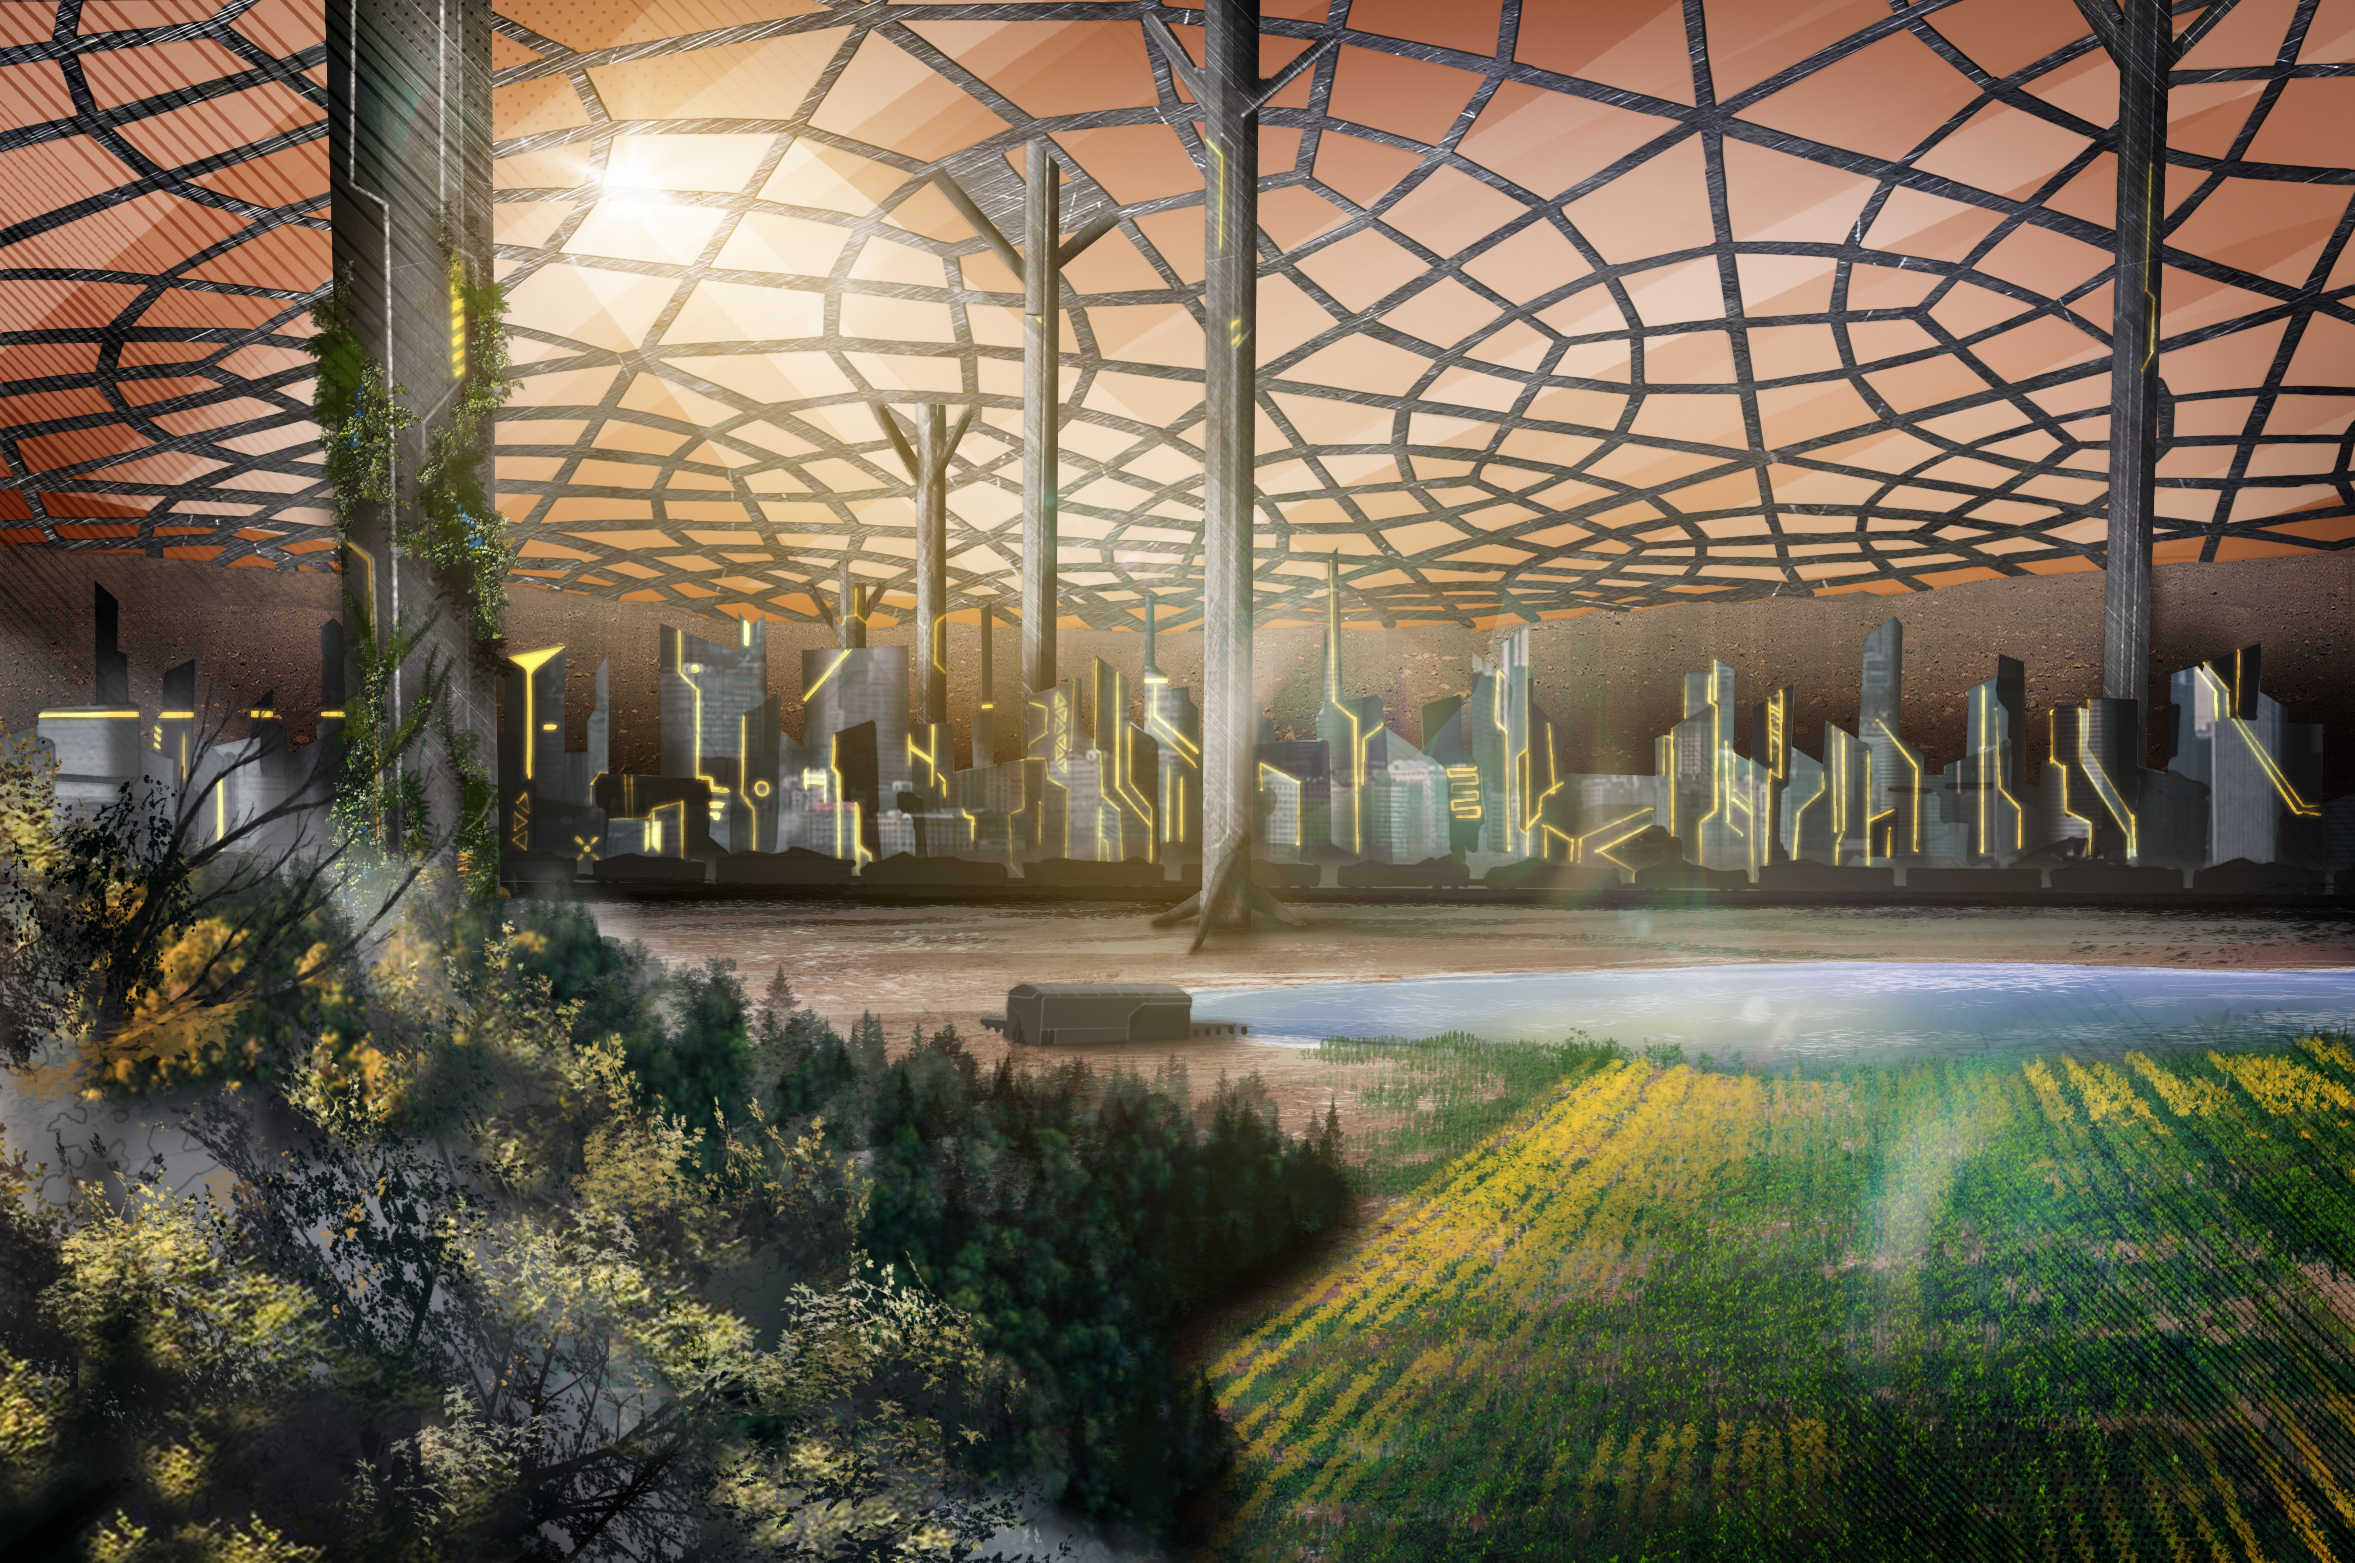
\includegraphics[width=\linewidth]{art/terraformed_dome.jpg}
    \caption{Artist's rendition of the goal, the terraformed crater.}
    \label{fig:terraformed_dome}
\end{figure}

%---------------------------------------------------------------------------------
%	SECTION 1: TECHNICAL DESIGN
%---------------------------------------------------------------------------------

\section{Technical Design}
\label{sec:technical-design}

Due to the presence of high transport costs from Earth and the inherent risks of delays in the transport of critical imports; for human life to survive and ultimately flourish on KCSAR, the colony must be highly self-sufficient and operate as a close to autarkic entity. To achieve this, cost-efficient manufacturing processes of essential bulk materials are critical. In this section, we outline the engineering that underpins these processes, first dealing with necessities for human life, namely, power, air, water, and food; then addressing economic necessities and focusing on bulk materials, mining, consumables and the internet. Within each of these sectoral subsections, we introduce the structure and scale of resource dependence, before analysing the key production pathways (chemical, engineering, manufacturing) needed to achieve essential self sufficiency.

\subsection{Absolute Necessities of Life}

Given the resource scarcity, the production line for a number of essential necessities proposed here, are designed to operate synergistically with one another. This maximises productivity while enabling a futures market to arise from the multiple production processes with distinct production curves. The resulting overall system, therefore, is robust, efficient, and responsive to any market turbulence.

\subsubsection{Power and Thermal Design}
\label{sec:necessities_power}

We begin with power consumption and generation, as all subsequent processes depend upon it. KCSAR requires on average $\approx$1GWe (with an upper limit of $\approx$3GWe) to sustain life for one million people. KCSAR’s complete power generation model can be described as an interconnected system that encompasses thermal and electric power generated via two different processes: (1) a nuclear base-load plant that produces 12GWth power output from an integral fast-spectrum two-fluid molten-salt reactor operating at 750\degree{}C, of which, 4GWe power is obtained from a series of in-situ mass-producible low pressure turbines; and (2) a cryogenic peaker plant that produces 4GWe power output derived from a cryogenic energy storage system (CES) that stores energy in the form of LN2, with capacity of 96GWh, providing the energy requirements to meet peak demand. As seen in figure \ref{fig:power_diagram}, this two-way system maximises the productivity of the power generated, by interacting with other energy-producing processes. For example, during periods of peak demand, the risk to grid instability arising from network overload is ameliorated through the usage of a cryobattery, and, during periods of minimal demand, the excess thermal output can be redistributed for other uses, such as powering the chemical market to increase the production of bulk goods, or recharging the cryobattery. This system relies crucially on the presence of a sufficient heat-sink, due to the heat density of the molten salt reactor design, and the particularities of the Martian context. The absence of large bodies of water and a thick atmosphere make thermal rejection particularly problematic. Opportunistically, however, KCSAR is located on water ice, which provides the necessary heat-sink needed for the long-term viability of the system.

The reactor itself is an integral design made up of standard high temperature materials, and houses a single crucible that contains the entire assembly. It uses Hastalloy-N disposable fuel pins, which are filled with a fuel salt mixture that comprises plutonium and U238. These pins are the only superalloys that are required to be produced and shipped from Earth. Since it is a fast spectrum reactor, there is no requirement to isotropically separate lithium for the FliBe mixed fuel salt to maintain acceptable neutronics. By using this two fluid contained pin design, we can separate the fuel to simplify the reactor maintenance and construction, and therefore avoid the complications arising from (1) the potential condensation of fission products, and (2) the production of Xenon and Krypton. Additionally, as a liquid fuel, it can be burned more completely because the standard Xenon intercalation problems found in MOX are not present. The chloride based coolant salt is then wrapped in a Thorium salt ‘blanket’, allowing it to be bred for U233 via Pa for use in nuclear thermal vehicles, along with Kilopower style stationary reactors for use in mining colonies and the like. By operating under low pressure Argon on Mars, the usual corrosion problems associated with water or oxygen impurities in the fuel salt are eliminated. Overall, the reactor is designed to run at a 100\% capacity factor, with redundant heat exchangers and turbines, and at $\approx$100\% load factor between the electrical and thermal energy demands on the system, matching demand via a smart grid system \cite{Shultis2016}. 

The thermal energy generated by the reactor is converted to electricity via low pressure turbines that are manufactured on Mars. The benefit of using these turbines over standard high-pressure turbines is that they do not require precision manufacturing or advanced metallurgy, allowing them to be mass-produced in-situ, on Mars. Inputs into the thermal distribution system are a combination of the rejected heat of the reactor fluids themselves, absorption chillers, and waste heat from chemical industrial plants, which are then used to generate various output loops at chemically useful temperatures, as well as a final rejection loop for any heat that is too low grade for industry, which is used to melt ice and for district heating. The combined heat and power system (driven largely by the reactor’s excess thermal energy), produces ‘plant heat’ that can be used within various chemical plants to develop other essential goods such as food (refer to section \ref{sec:necessities_food}) and fuel (refer to section \ref{sec:necessities_bulk}), while also providing the necessary heat needed for natural ecosystems to thrive (e.g. by facilitating the growth of cold water fish and algae). Furthermore, waste heat from the reactor is also capitalised on to form large inlets of liquid water by heating the ice (an essential resource for life, that is discussed at great lengths in section \ref{sec:necessities_water}). A second purpose of the waste heat from the reactor, is that is can address the challenge of bulk cooling on Mars. By using a series of absorption chillers, such as a LiBr absorption chiller that produces water at 2\degree{}C, or an ammonia absorption chiller that produces a chilled methanol loop at -30\degree{}C, the waste heat has useful properties that allow for the chilling of objects below the temperature of the inlet as required.

\begin{figure}
    \centering
    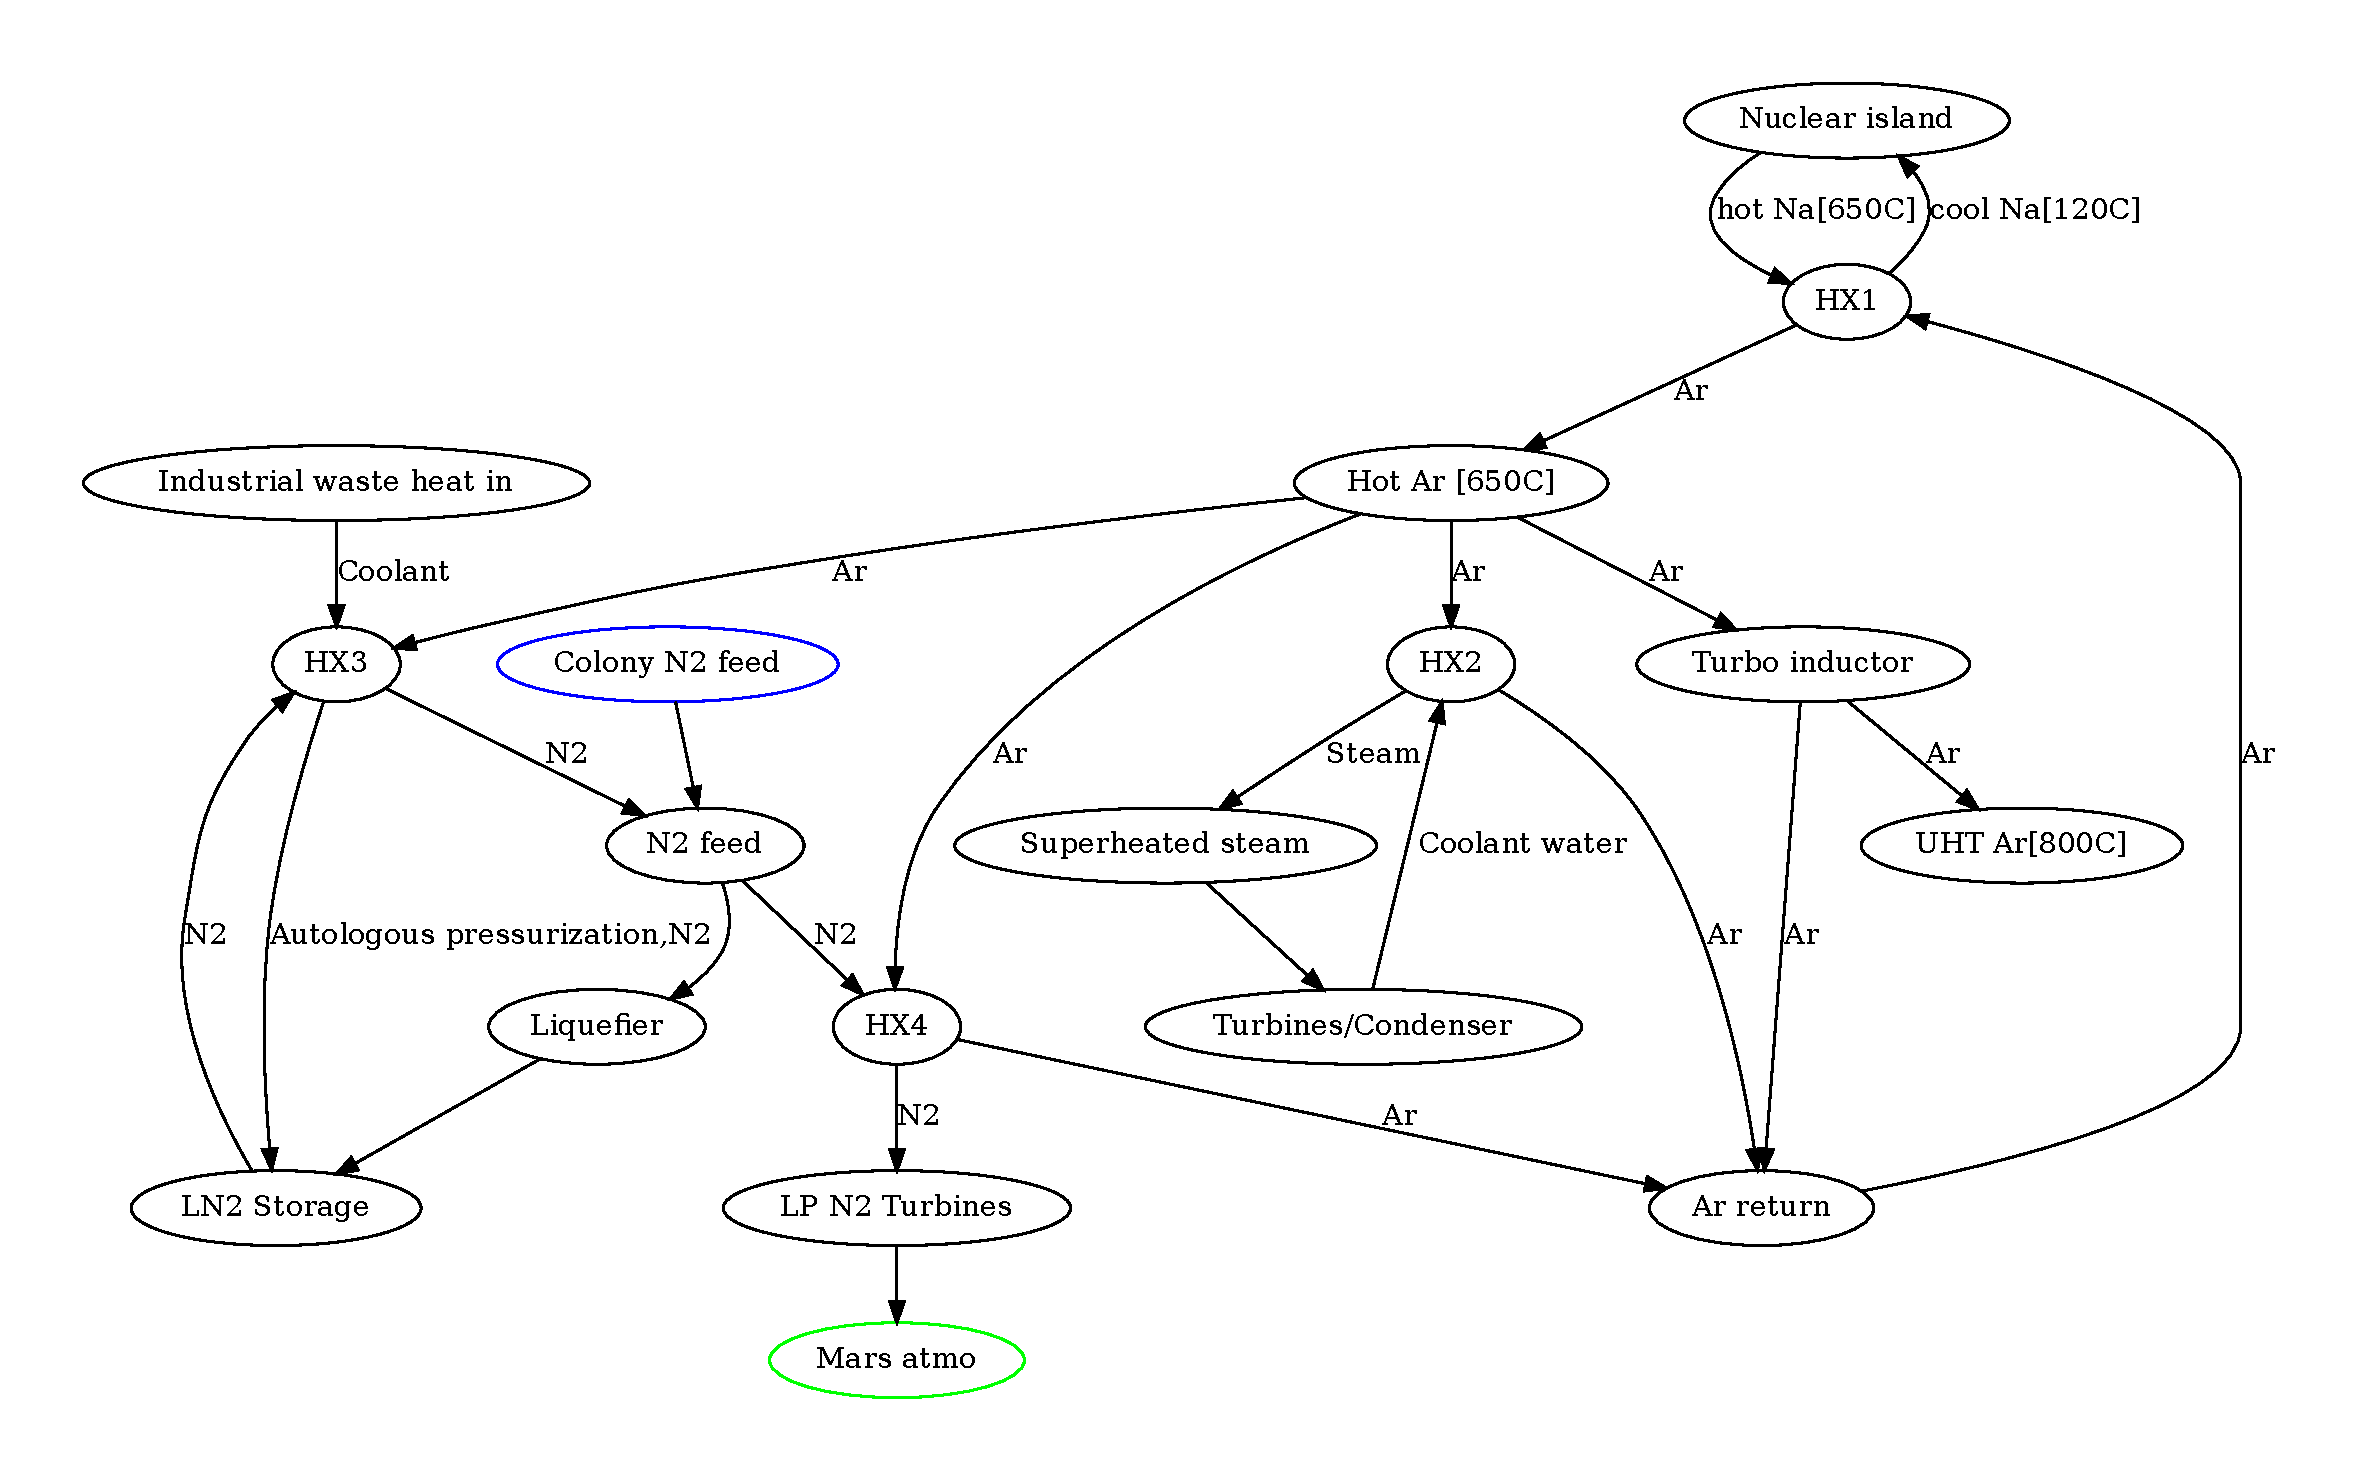
\includegraphics[width=\linewidth]{figures/fig_power.pdf}
    \caption{Reactor thermal distribution diagram}
    \label{fig:power_diagram}
\end{figure}

Finally, any excess energy produced is stored within a cryogenic battery \cite{Hogberg2018} made up of LN2, that is used as needed to meet peak energy demands. LN2 is heated by industrial waste heat to (1) form high pressure N2 that turns the locally produced low pressure turbines, and (2) provides the means to both operate the LN2 turbopump and pressurize the LN2 tanks. To ensure that the cryogenic tanks remain chilled, a novel approach to radiative cooling is used. A solar absorber that is made up of an undoped Ge film, below an epitaxial Ge02 scratch resistant layer, is used to create a shading mechanism for the black body radiative cooler through a ZnSe window. An anodized black-body radiator in a dewar then acts as a heat exchanger for He, which enters through the bottom and is cooled to create the cold loop that chills the cryogenic tanks. The chilled He can then be used to either liquify boiled off gasses, or cool liquid gas as required. Given that the thin atmosphere of Mars radiates less IR at night as a black body, it is relatively simple to build larger vacuum chambers to support this system as needed \cite{Chen2019}. Some of the key benefits of using cryogenic batteries are: (a) they provide a sacrificial LN2 blanket that reduces the loss associated with the relatively valuable LO2 and CH4; (b) economically, it creates elasticity in the supply of electrical energy, by ensuring demand for electricity from the reactor and offering the capacity to redistribute it as needed; and (c) since there is a market for both reactor heat and power that can be converted into each other, the fungibility of these resources softens the demand curve for each, ensuring a stable market equilibrium.

While developing a colony in the bitter cold of the Martian pole may seem like a brutal trade off for easily producible energy and living space; it is less brutal than one would initially assume. Most of the colony exists within the glacier in domes that are designed with striking similarities to Igloos, in that they take advantage of (1) the insulating properties of ice and (2) the large thermal mass of the glacier, in order to maintain a reasonable temperature. Furthermore, at the surface, even though the temperature itself may be below -100\degree{}C, the low pressure environment reduces convection losses, while the CO2 atmosphere reduces conduction losses (compared to an N2-based environment). This means that as a frame of reference, the engineering problem of heat conservation is actually comparable to the equivalent of much warmer temperatures on Earth.

\subsubsection{Air and Atmosphere}
\label{sec:necessities_air}
%For the westinghouse design, the reference is wrong and I can't find a new one.
% Old text was "a Westinghouse \cite{ErhongDuan2011} style sulfuric acid decomposer"


% Modular decomposer citation: 10.13182/NT12-A13551

Next, of primary concern is the supply of the chemicals that form the basis of survival: air and water. In this section we explore the atmospheric conditions required for life to permeate Mars, dealing first with oxygen, the foundation of human life. By far, the easiest method to produce oxygen on Mars is via photosynthesis. However, the challenge is that the supply needs must be determined long in advance (via building farms) and is reasonably unreliable. To mitigate this issue, cryogenic oxygen that is kept cold via the cryobattery’s LN2 that we introduced in section \ref{sec:necessities_power}, offers a short term solution to stabilizing the supply. In the medium term, or where farming is impractical, a Zn/S/I thermochemical cycle \cite{YanweiZhang2013} is proposed to produce oxygen from water at a reasonable cost, using a turboinductor heat pump to efficiently provide optimal operating temperature \cite{JohnBucknellVideo, 2013Dujarric}. The reactor would use an electrochemical bunsen stage \cite{YanweiZhang2016}, with a modular decomposer akin to [citation here ], to save on complexity and cost. Similar designs would also be used to produce O2 from CO2 by omitting the HI decomposition stage, making them suitable for other things, such as life support on mining outposts, powered by kilopower style power plants. A further benefit to Zn/S/I systems is that they both produce the syngas needed for the direct reduction of iron, and consume the water/CO2 generated from the reduction. The interrelationship of these processes used to generate atmospheric conditions are displayed in \ref{fig:atmo_diagram}. 

Given that KCSAR’s atmosphere is primarily made up of low pressure Oxygen and Argon (Argox), the photosynthetic farms can capitalise on a CO2 enriched atmosphere, which can produce an enriched Argox fraction when processed, by recycling the CO2 back into the farms. This  Argox fraction underpins  the city’s atmosphere, supplemented as needed using Air Handling Units(AHU) which maintain total pressure, along with things like temperature, the partial pressures of O2/CO2, and humidity. To ensure that excess atmosphere does not pose a serious threat during events such as a fire, a reject line is used; and any water produced via dehumidification is rejected via a drain line. Another potentially lethal threat on Mars, is the issue of dust, which can lead to health problems such as chronic silicosis. To address this issue, cyclonic filtration with a second electrostatic stage is employed as a scalable way to remove possibly harmful small particles. Provisions must also be made for potential atmospheric failures. Respirators that enclose the ears and eyes are maintained at regular intervals to ensure that citizens have enough time to return to safety if they are unable to access a full pressure suit. Atmospheric monitors and alarms are built into each AHU that operates if pressure falls to a dangerous level, or if the partial pressure of oxygen or CO2 moves outside of safe bounds. The potent odorant Ethanethiol is added to the emergency habitat pressurisation lines, to provide a warning for underpressure and hypoxic situations. While above the ice, depressurization due to pinhole leaks is a major concern, under the ice, the primary hazard is hypoxia or toxic gas buildup due to fire or a chemical leak that rapidly replaces the atmosphere with high pressure, unbreathable gas. An overpressure system within the AHU’s allows for them to rapidly vent out the excess gas, preventing the problems associated with overpressure.

\begin{figure*}
    \centering
    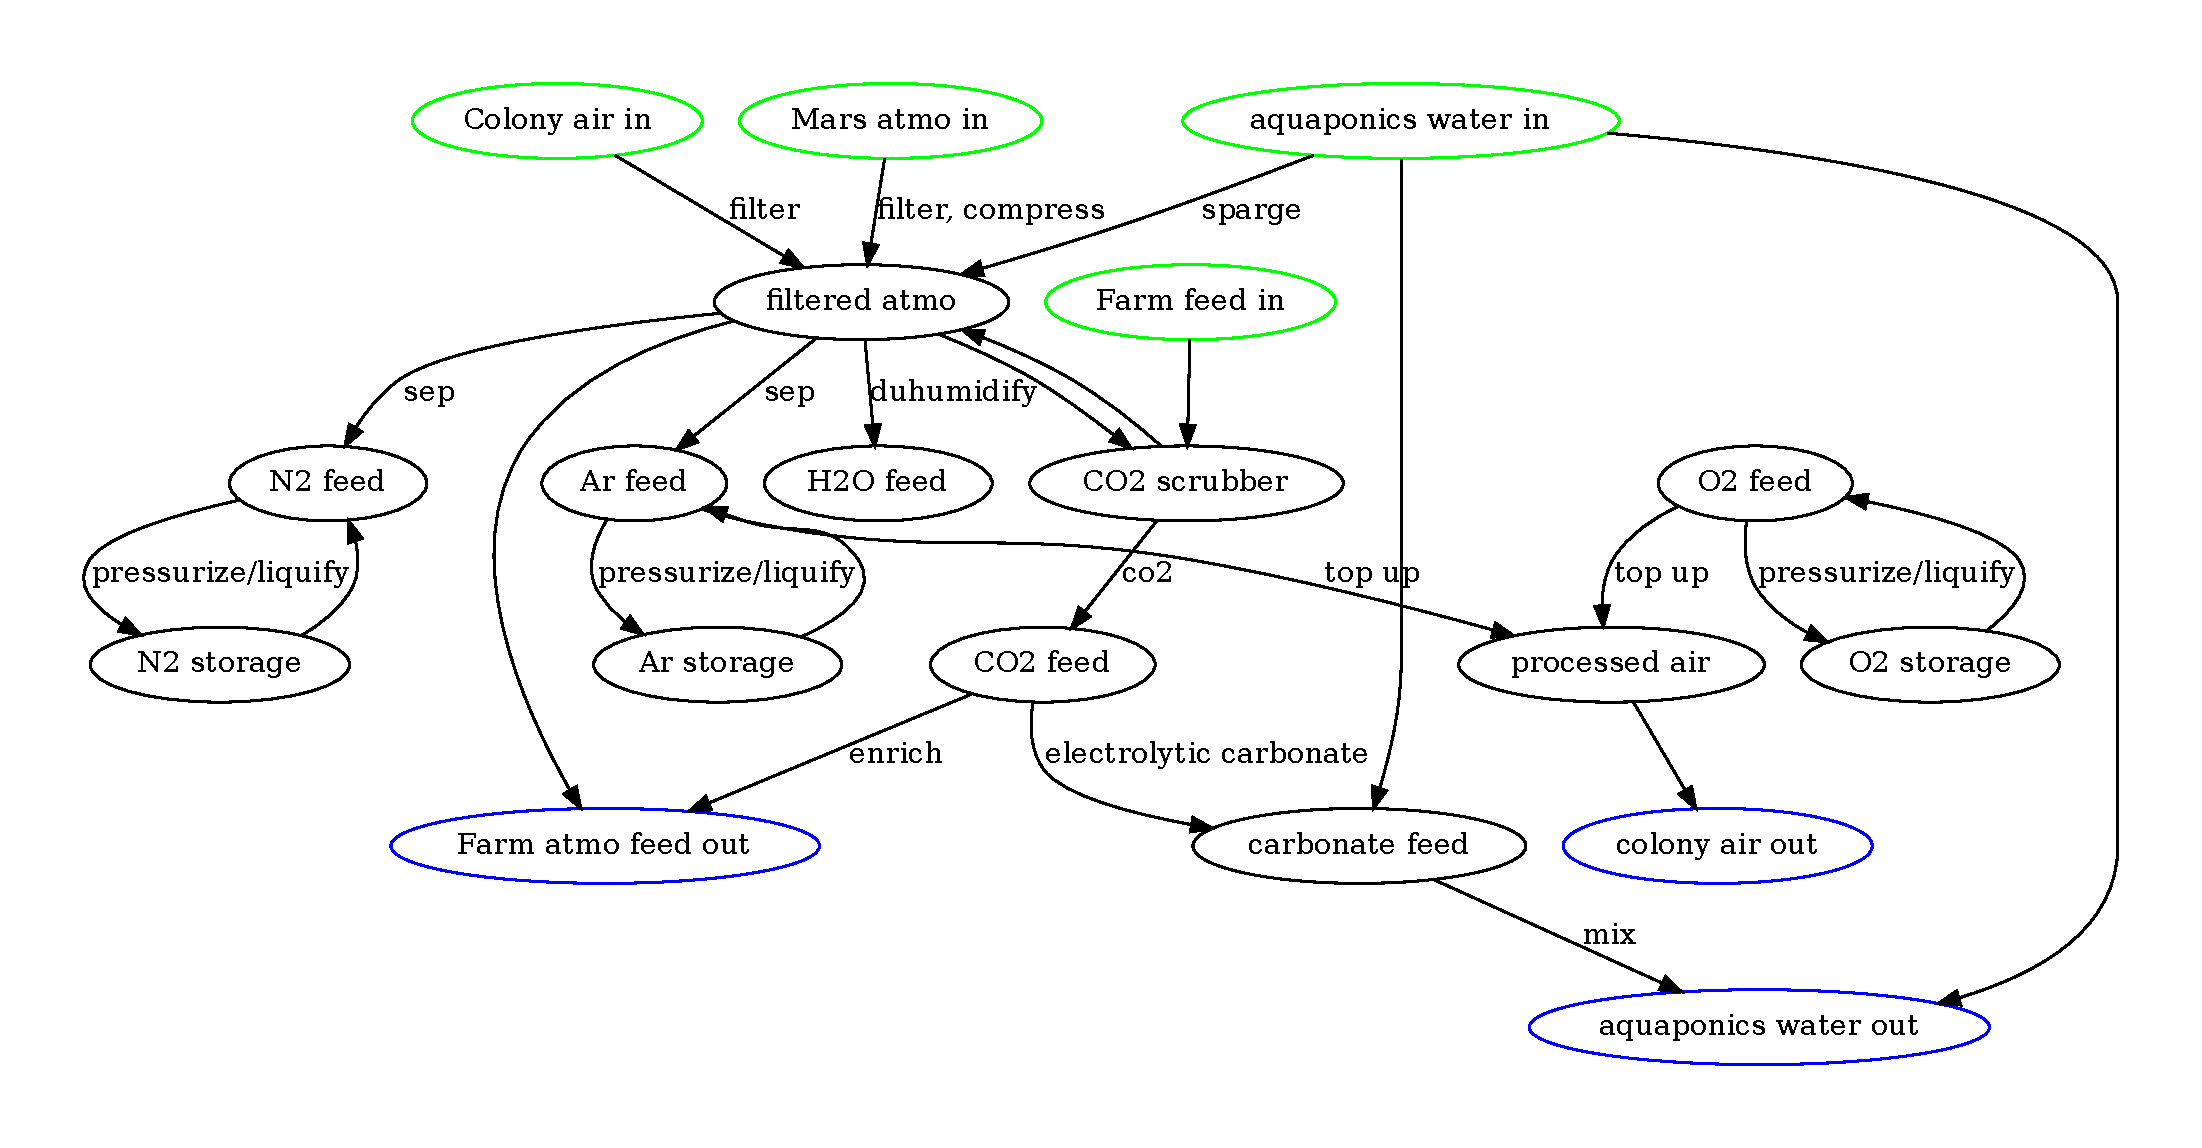
\includegraphics[width=\linewidth]{figures/fig_atmo.pdf}
    \caption{A high level diagram of the flow of atmosphere between the settlement, farms and industry}
    \label{fig:atmo_diagram}
\end{figure*}

\subsubsection{Water}
\label{sec:necessities_water}

Extending on our treatment of air, access to liquid water is equally critical, and, once again, the value proposition of settling on the Korolev crater presents itself. Since KCSAR is located and built into water ice, it is surrounded by an accessible water source if heat energy is available. To heat the ice, KCSAR capitalises on the heat exchangers from the reactor proposed in section \ref{sec:necessities_power}. The high temperature output from the reactor produces waste heat that leads to the formation of local ponds, which, over time, transforms into an inlet of accessible liquid water, particularly as the heat dissipates through the surrounding ice walls. While the lake water is not initially potable, a novel two-stage temperature swing solvent extraction (TSSE) process \cite{ChanheeBoo2019}, provides an effective solution for the bulk recycling of water. In the first stage, the solvent Diisopropylamine (DIPA) is heated to absorb water from the raw water inlet until it is saturated. It is then cooled so that the DIPA rejects excess water and forms an aqueous layer that can be removed \cite{CRC_84Ed}. In the second stage, Diethyl ether (Eth) is used to extract the remaining DIPA from the extracted water. Given that Eth is mostly immiscible with water, and has a low boiling point and high vapour pressure, it is easily extracted. Finally, the water is treated to maximise its safety using: (1) activated charcoal filtering (2) NaOCL is added as a disinfectant and (3) a buffered mixture of common ions to ensure that (a) the pH of the water remains slightly alkaline, (b) metal pipes passivate properly, and (c) leeched metal ions are insoluble. Minerals are also added to improve nutritional outcomes, such as NaF for dental health.

TSSE is an attractive candidate process because (1) it only requires simple mechanical equipment, and (2) it runs on low grade waste heat, at standard pressure, and with mild reaction conditions. This is preferred to more standard reverse osmosis systems that rely on high precision semi-permeable membranes that are complex to manufacture, and that require energy intensive high pressure pumps. Moreover, this TSSE process can internally recycle the low-grade waste heat using a recuperator, which makes it highly energy efficient, and only requires chemicals and materials that are easy to produce in-situ. This ensures that the system is easily scalable as the population grows \cite{ChanheeBoo2019}. Particularly as the population grows, recycled wastewater is therefore the most efficient primary source of water and only supplemented by the energy-costly process of converting large blocks of ice into water where necessary. A relatively simple recycling process is used for 'greywater', produced from sources such as showers on Mars. Greywater does not contain harmful biological organisms, and therefore, the water can be passed through a simple filter stage and fed back into the aquaponic loop that we describe in section \ref{sec:necessities_food}. 'Blackwater', by contrast, does contain harmful organisms that need to be removed, but also contains nitrates and phosphates that make it a good fertiliser. Thus, by diluting blackwater with greywater, and using NaOCl and thermal processing to sterilise it, it is also capable of being utilised in the aquaponics loop. This overarching synergistic water treatment process is laid out in figure \ref{fig:water_diagram}.

\begin{figure*}
    \centering
    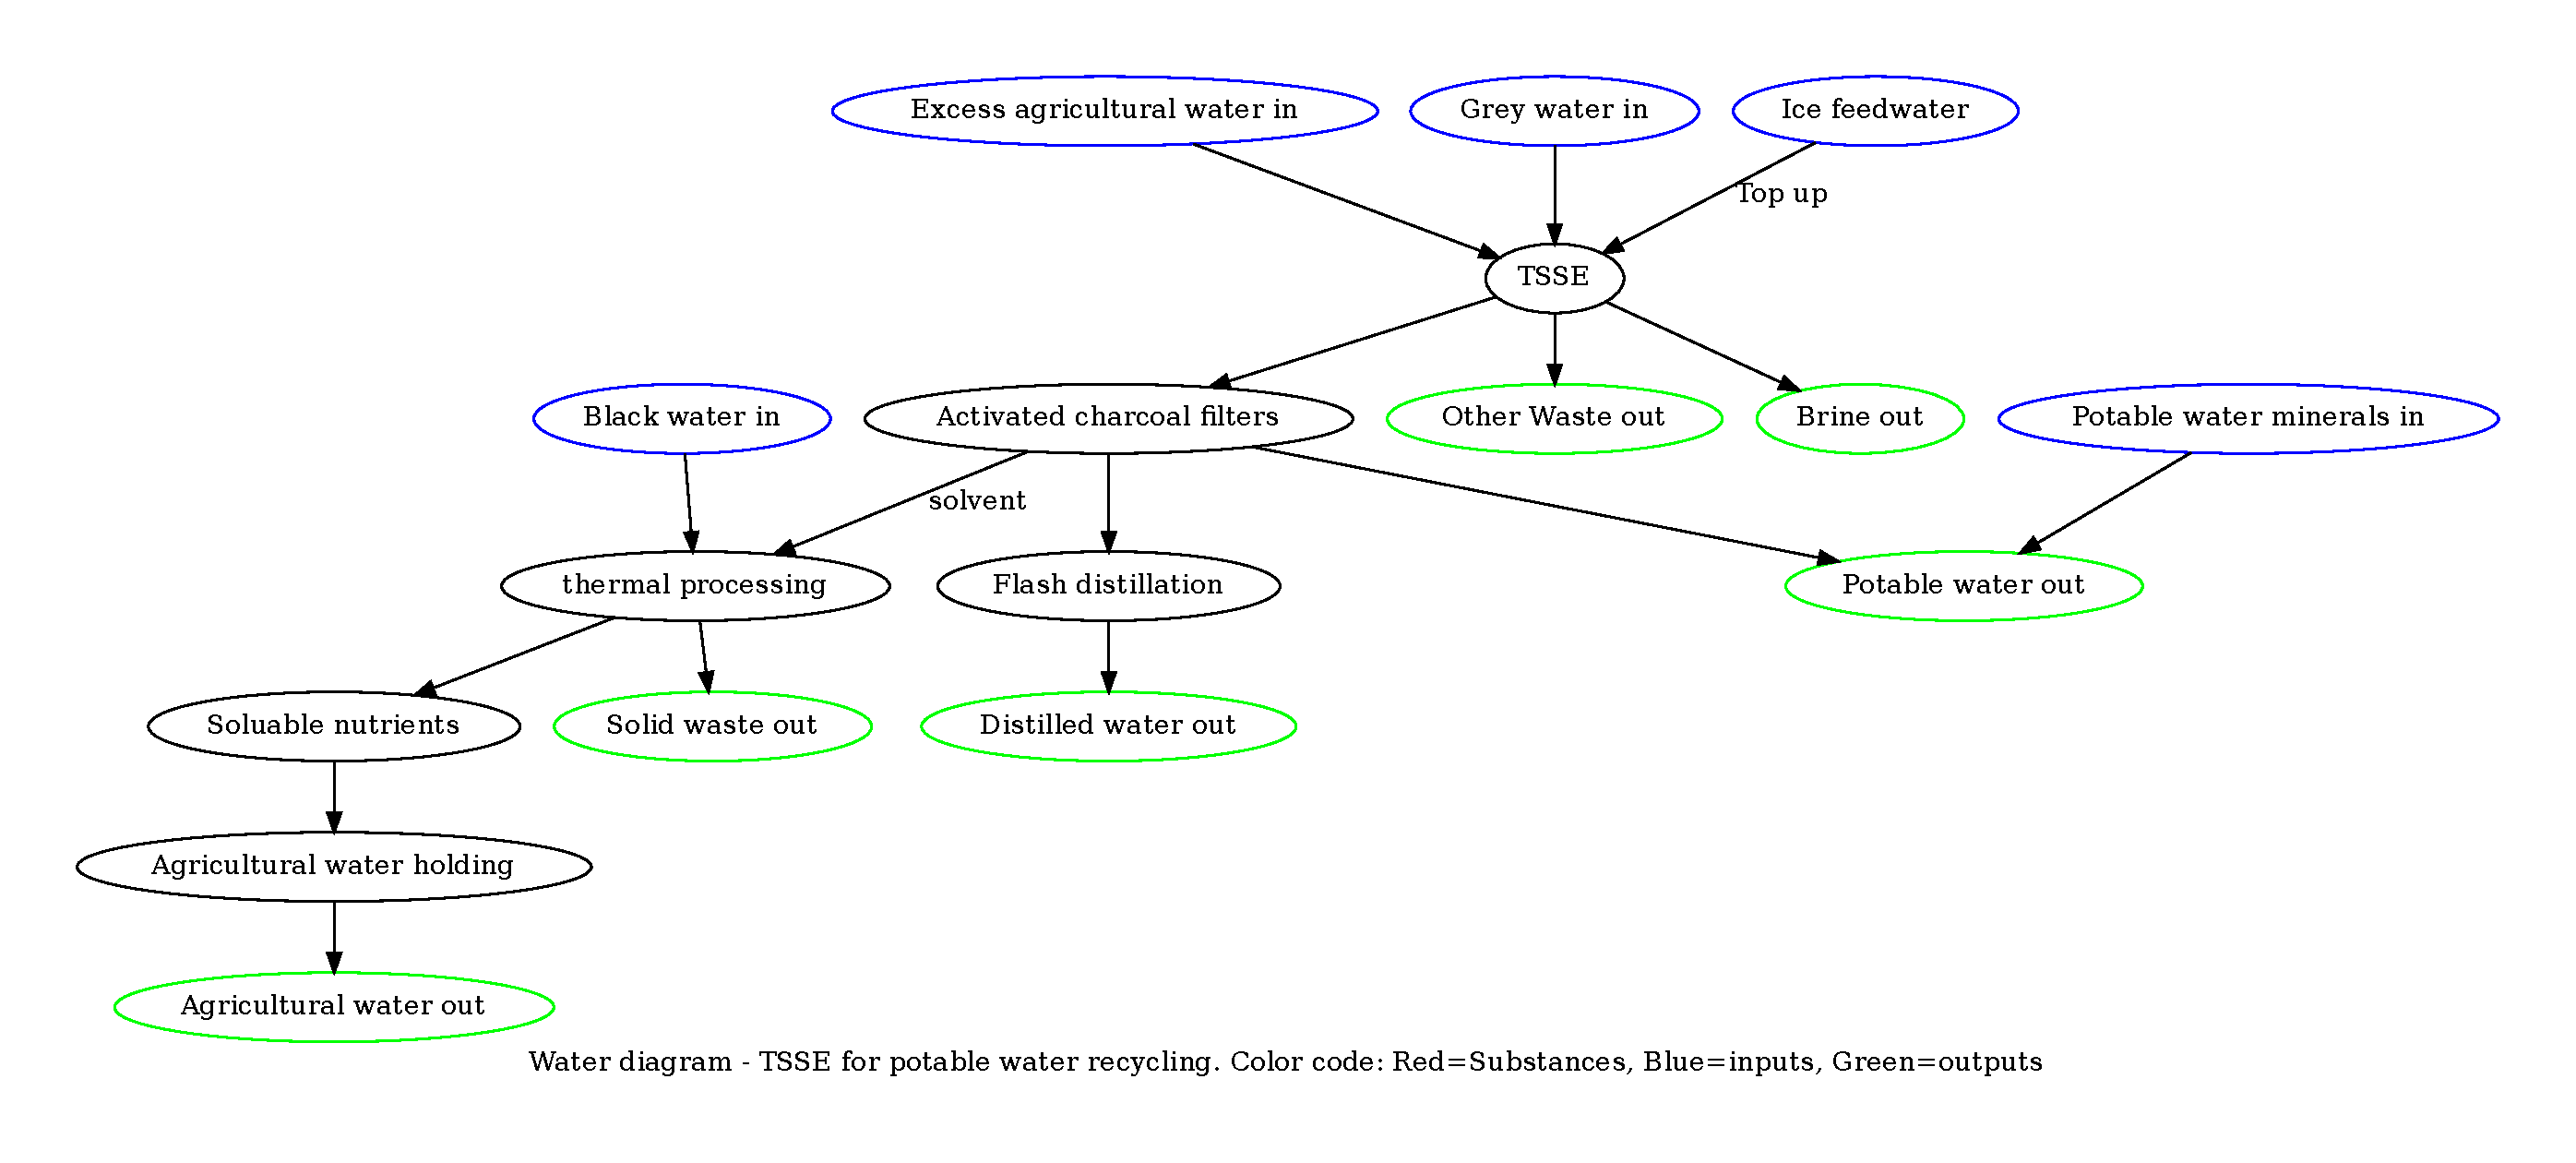
\includegraphics[width=\linewidth]{figures/fig_water.pdf}
    \caption{The artificial water cycle of the settlement. Colors: Blue are inputs, Green are outputs.}
    \label{fig:water_diagram}
\end{figure*}

\subsubsection{Food}
\label{sec:necessities_food}
 
For an isolated community such as KCSAR, maintaining food security is vital. Producing a sufficient quantity of cost-efficient, nutrient-diverse foods, while maintaining efficient supply lines, is a prerequisite for the sustenance of life. In this section, we outline the artificial ecosystem that provides a varied diet for the citizens of KCSAR, building from the simplest (and most cost efficient) food sources, to the most complex luxury goods. Given the complexity of maintaining food security, we have divided the treatment of this section into two sequential parts, answering the vital questions of: (1) What chemical processes are needed to enable the production of food? (2) How then, do we mass produce the food in a sustainable way?

\paragraph{The Chemical Pathways Required for Food Production}

Edible industrial products are an extremely cheap food source, and underpin food security, even when there are disruptions in the supply of other nutrient sources. They serve a dual purpose, forming inputs for the biochemical industry discussed in section \ref{sec:necessities_bulk} once they are processed. For example, edible glucose is converted into plastice and protein into ammonia. These edible industrial products are primarily produced in ditch-style farms and grass farms. Ditch-style farming involves injecting water into an earthen dam and covering it in a layer of Oleic acid to protect it from the low pressure / temperature of the surface, so that optimal growth conditions are maintained. Figure \ref{fig:oleic_acid_bp} shows the depth of Oleic acid needed to enable growth. Below the red line, no economically useful growth is possible. Between the red and orange lines, many forms of algae can be grown in useful quantities. The two green lines show the range of optimal growing conditions for Spirulina, a useful cyanobacteria that has adapted to very warm water environments. Within this range, it grows rapidly, producing nutrient rich biomass that feeds both people and animals. The cost efficiency of producing candidate algaes is routinely reviewed to create an appropriate environment for rapid growth. This is achieved, for example, by rotating the crop, or adjusting the depth of the Oleic acid. Since Oleic acid is produced from biomass and is needed for biomass production, this forms a feedback loop that limits the growth of farming over time.

\begin{figure}
    \centering
    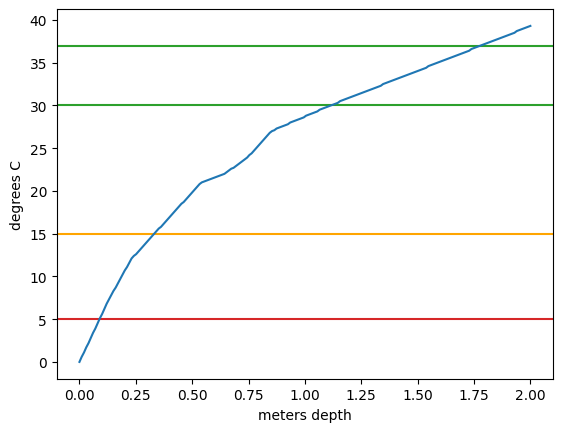
\includegraphics[width=\linewidth]{figures/fig_bp.png}
    \caption{Depth of oleic acid vs. maximum water temperature}
    \label{fig:oleic_acid_bp}
\end{figure}

The primary obstacle to ditch-style farming is the method of gas perfusion. There is no viable natural path to enable CO2 and N2 from the Martian atmosphere to reach the aqueous layer for biosynthesis. Hence perfusion stations are used, replacing consumed dissolved gasses such as CO2 and possibly N2, and then extracting the dissolved O2. 

Another form of farming - mushroom farming - is also used to catabolise otherwise indigestible biomass into nutrients for future farming. This removes insoluble products that cannot be ground into a colloid and fed into hydroponic systems. Mushroom farming requires O2 and waste biomass that can be seeded with spores to form edible mushrooms.

Given that nitrogen is critical to facilitating plant growth across the farms, either atmospheric nitrogen, or the artificial urea derived from the haber process described in section \ref{sec:necessities_bulk}, will be used as a nitrogen source. While the N2 found within the Mars atmosphere is cheaper to use and requires less processing, its primary drawback is that it results in slower growth. Artificial urea, on the other hand, is more effective, but subject to market fluctuations in the industrial price of urea.

\paragraph{The Sustainable Mass Production of Food}

Whilst building robotic greenhouses that can grow standard crops is a daunting technical challenge, automated farming of light grasses and particularly Miscanthus Giganteus (‘elephant grass’) have been reliably implemented. On KCSAR, this procedure is replicated to produce a cost-efficient source of industrial glucose. Small modular greenhouse sections are fused together and filled with low pressure CO2-enhanced atmosphere. Quantum dots are employed as a layer on top of the greenhouse membrane to increase quantum efficiency by downconverting light that is unsuitable for the grass, such as UV light, into light that is most effective for photosynthesis. The growth beds resemble traditional hydroponic growth beds and are made from processed, crushed regolith. These are robotically mowed, with the farmed grass cracked into glucose by cellulases. Using a similar approach, hydroponic gardens will be used to grow more traditional foods including vegetables, grains and spices. Due to the complexity of harvesting, hydroponic gardens require laborers and a shirt-sleeve environment, making their output substantially more expensive.

Aquaponic farming is also used to supplement the Martian diet with fish and aquatic lifeforms. Aquaponic farms are contained within large bioplastic boxes with an Oleic acid cap, placed in segmented areas cut into the ice. The box acts as insulation, keeping the water warm and separating out the nutrient-rich (particularly phosphate-rich) water that accelerates the growth of cyanobacteria and algae, from dilute water. As these organisms are at the bottom of an artificial food chain, the speed of their growth is highly correlated with the supply of fish of various kinds, that are a staple of the relatively wealthy. 

While relatively expensive, meat is also sufficiently cheap to supplement the diets of most households with varying frequency. Battery poultry, rabbits and similar livestock are the primary source of meat as they may be grown relatively cost efficiently, rapidly and in confined spaces, and they are farmed for eggs and meat. A substantial amount of farmed meat is processed, with cellulose ‘padding’ added (such as in chicken nuggets) to make it more affordable for consumers. 

Yeast, farmed in bioreactors, is used to grow bulk substitute animal proteins, such as albumin from eggs and caseins from milk, from industrial feedstock. This allows for the creation of cheaper substitute products, such as artificial egg whites, as opposed to far more expensive chicken eggs. These are also mixed with processed meats or fish to form more complete processed foods, or even added to semi-natural pathways to create, for example, real cheese out of artificial milk \cite{Pandya2017}. Similarly, using artificial gluten and eggs enables the colony to bake bread and make pasta, which would otherwise be infeasible, thereby allowing for a more varied diet.

In the highest price bracket, are the imported foods from Earth that are infeasible to replicate on Mars such as chocolate and coffee, depending on demand. Where possible, these foods are produced using a mixture of local and imported ingredients. For example, chocolate is produced from combining artificial oils and bulk glucose produced on Mars with cocoa that is imported from Earth. To improve food flavour in a relatively inexpensive way, some spices are engineered chemically (such as simple esters) and biologically (such as limonene, linalool, among others), which makes the food more palatable to those familiar with traditional foods consumed on Earth. Spices that cannot be produced through these methods are imported from Earth. The change in the relative costs of ingredients provides the impetus for culinary innovation and the growth of a distinctive Martian cuisine.

While these diverse farming practices meet most of citizens' nutritional needs, some nutrient deficiencies arise because foods that are high in particular nutrients are difficult or expensive to produce. To address the possibility of widespread deficiencies and resulting health impacts, many foods are fortified with artificial sources of Vitamin C, Vitamin D and Iodine.

% TODO: Didn't find a suitable place for this in food, needs to be re-evaluated:
%------------------------------------------------------------------------
% Reactor plant heat can also be used to produce methanol to farm methanotrophs, providing a reasonably direct mechanism to convert nuclear power to food or other products.
% For example, CO2 separated through amine or ionic liquid scrubbing \cite{Lotto2018,StephenYates2016} is used a chemical input

\subsection{Economic Necessities of Life}

In the previous section, we outlined the basic processes needed to sustain human life on Mars. In this section, we analyse the processes necessary to sustain a stable, working economy that can maintain those basic processes and provide for human consumer 'wants' as well as needs. As before, cost efficiency and stability are the primary motivation for selecting particular production and maintenance processes. 


\subsubsection{Bulk Materials}
\label{sec:necessities_bulk}

The next most important chemical pathways are those that are economically essential for survival - the production of plastics and other bulk products. For simplicity, we have compiled a list of useful bulk products that are producible on Mars in table \ref{tab:bulk_products}. A key consideration in the robust production of bulk materials is that there are multiple pathways with different production functions. As an example producing Aniline in a bioreactor requires very little in the way of capital outlay and so is easily scalable, but has a higher marginal cost per ton than building a dedicated plant to aminate phenol. A market that includes both, then, along with a robust futures market in industrial products, is able to produce cheaply, while scaling rapidly, in order to robustly meet market demand.

Another key consideration is that while some biological processes are directly useful, such as the production of bioplastics, artificial oils, Vitamin B12 and the like, some are not. In those cases biological processes need to be augmented with industrial chemistry to produce useful products, for example producing acetaminophen from biosynthetic Quinone, Or Nylon from synthetic Adipic acid \cite{WeiNiu2002}, Rubber from ethanol \cite{JunmingSun2011} (via isobutene), Epoxy from phenol, THF from processed plant sugars \cite{ShuoChen2018}, etc. All key components of a modern industrial economy.

\begin{table*}
\label{tab:bulk_products}
\centering
\begin{tabular}{|m{4cm}|L|}\hline
\textbf{Product} & \textbf{Production Process} \\\hline
Benze and its Derivatives &	BXT \cite{QingfengChe2019}, along with Phenol \cite{2001Gibson}, Quinone \cite{NingqingRan2001}, Aniline \cite{Pharkya2020}, among others \cite{JianLi2017} are produced from biomass, either directly through digestion, or via catalytic conversion of biological precursors. \\\hline
Ammonia & This is produced through the combination of a catabolic degradation of protein \cite{KwonYoungChoi2014} and a low pressure advanced haber reactor \cite{BosongLin2019} utilising plant heat.\\\hline
Ethene & This is produced from bioethanol.\\\hline
Sulfuric / Phosphoric Acid &  Generated from acid gases produced in the metal refining process observed in section \ref{sec:necessities_raw}. \\\hline
Nitric Acid & This is produced by the oxidation of ammonia.\\\hline
Methane & This is produced through the sabatier \cite{JohnBucknell2014} process using reactor plant heat, along with bioalkane cracking \cite{2004JoseComas, XWang2002}.\\\hline
Hydrogen &  This is produced from water via the S/I cycle, via steam reforming of methane \cite{JianhuaTong2006}, as well as via ammonia decomposition. Storage of hydrogen chemically then allows for the non-cryogenic storage of bulk hydrogen.\\\hline
Biomass & Biomass is mass produced in farms and in bioreactors. Specifically using Methanotrophs (Methylococcus capsulatus et al) fed on methane/methanol. \\\hline
Methanol, Alkanes & These are produced either chemically from Syngas via the Fischer Tropsch process and plant heat, or biologically from biomass. \\\hline
Syngas (H2, CO) & Syngas is produced via the Zn/S/I cycle (as seen in \ref{sec:necessities_air}) as well as through the gasification of Biomass \\\hline
Bioplastics & PHB, PLA and other bioplastics are produced from biomass. \\\hline
CO2 & CO2 is scrubbed from both the Martian atmosphere as well as artificial atmospheres through amine or ionic liquid scrubbing \cite{Lotto2018,StephenYates2016} as seen in figure \ref{fig:atmo_diagram}. \\\hline
NaOH, NaOCl, CL2 & These are produced in a standard chloralkali plant. \\\hline
\end{tabular}
\end{table*}

\subsubsection{Mining and Raw Materials}
\label{sec:necessities_raw}



\subsubsection{Factories and Consumables}
\label{sec:necessities_consumable}

One of the pertinent challenges that has pervaded much of our discussion of KCSAR, has been the idea that we need as many production lines to exist on Mars, given the high cost associated with imports. Given the availability of several bulk and raw materials, as reflected in sections \ref{sec:necessities_bulk} and \ref{sec:necessities_raw}, it is possible to develop and manufacture a range of specialised goods and consumables directly on Mars through the industrial sector - a key component of the Martian economy. To put this in context, importing complete objects such as computers is uneconomical, however, importing specific parts such as bare silicon wafers are relatively cheap, and can then be cost-efficiently transformed into packaged silicon chips, which are crucial for many processes. To support the development of bespoke capital and consumer goods, capitalising on 3d printing and other additive manufacturing processes may be important. However, it is worth noting that current 3d printing technology is prohibitive, due to the high cost and slow speed of 3d printing production, which forces KCSAR to rely primarily on more traditional manufacturing systems, at least until the technology further develops. Electrical Discharge Machining is used to produce injection molds for the mass production of high precision plastic parts made from bioplastics, such as PHB. Since factory systems are only partially automated, a sizable labor force is required to produce goods for the local population, and as a result, factory workers make up a significant proportion of the population.

\subsubsection{Internet}
\label{sec:necessities_internet}
The internet-based economy will be a key sector, both as an enabler of the export economy and in meeting domestic demand for communications and access to a forum for creating and sharing cultural products. The provision of stable, affordable internet service is therefore crucial. Long range laser are used for packet forwarding at the link layer, from an HEO outer shell of the Starlink constellation on earth and a similar constellation in HMO. Both constellations form Autonomous Systems, extending the internet advertisements of Earth and Mars to each other. Using the OSI model, this is then the L3 of the Martian internet.

The key issue is that, while packets can be routed and sent, the time delay prevents the use of higher level protocols. As such, KCSAR’s ISPs provide L4/L7 proxy services, similar to a traditional VPN service, that proxies connections on Earth via a proxy that understands the time delay. Existing CDN technology, such as NAPs is then used to allow large scale content providers (such as Youtube) to deploy content on Mars, with application-level changes that adjust for the increased spooling delays. An example of such a change is that movies or content created by artists that a user has ‘subscribed’ to are uploaded automatically, making them accessible from a local data center. If an individual clicks on a link that is not cached, they will be brought to the holding page, while the page is spooled from Earth and added to the local cache. Once added, it can be accessed almost instantly. ISPs provide caching proxies for most users but for security reasons, many companies run their own, renting capacity from Earth.

% TODO: Do we want to add anything about culture here?

\subsection{Services}

% NOTE: We might need some comment on services, but, if we are strapped for words, this could be integrated down as part of demographics / initial migrant selection etc

\begin{figure}
    \centering
    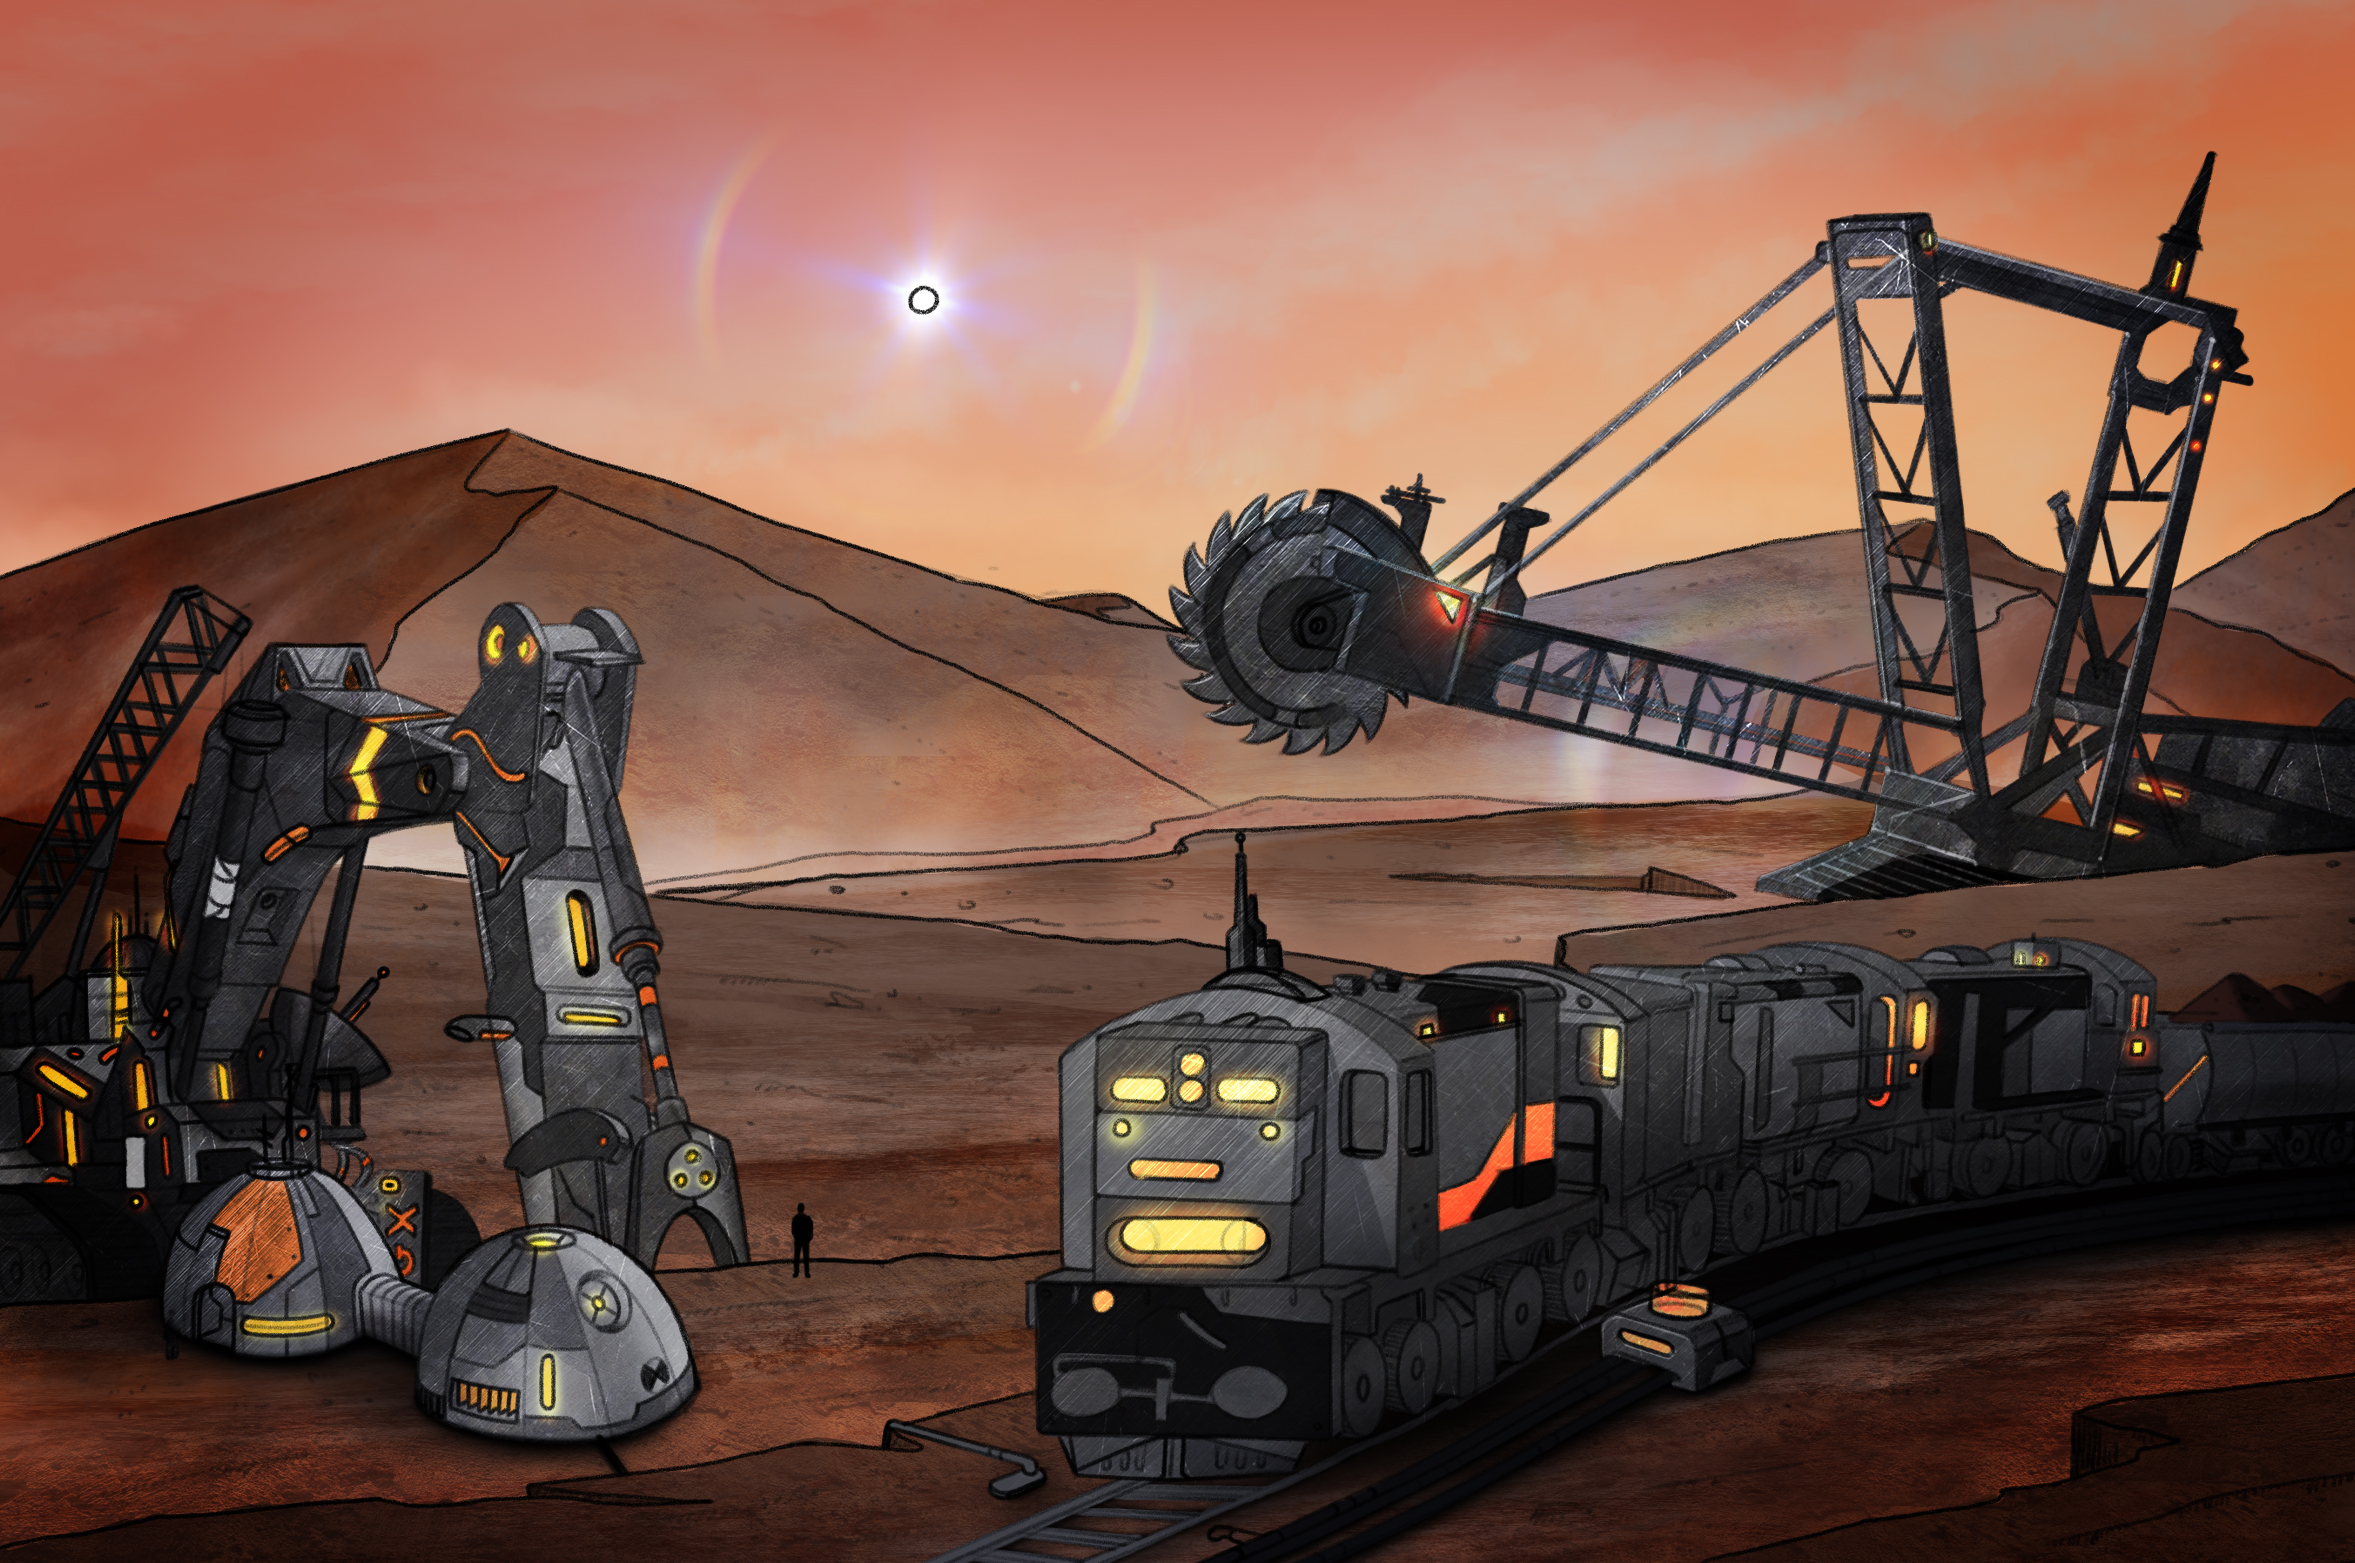
\includegraphics[width=\linewidth]{art/mining.jpg}
    \caption{Artist's rendition of the automated mines}
    \label{fig:mines}
\end{figure}

\begin{figure}
    \centering
    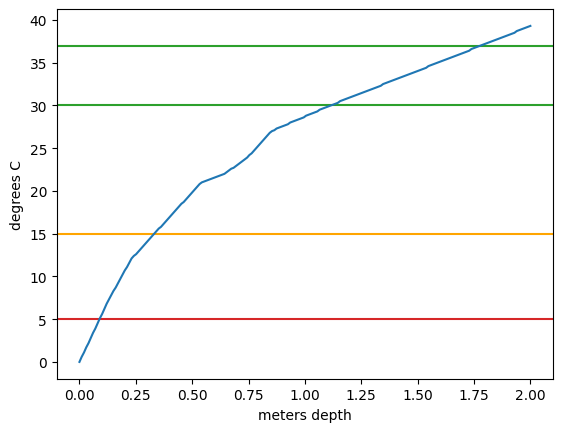
\includegraphics[width=\linewidth]{figures/fig_bp.png}
    \caption{Farm max temperature vs. depth}
    \label{fig:farm}
\end{figure}

% What does this chemical diagram show that isn't already provided in the text?
%\begin{figure}
%    \centering
%    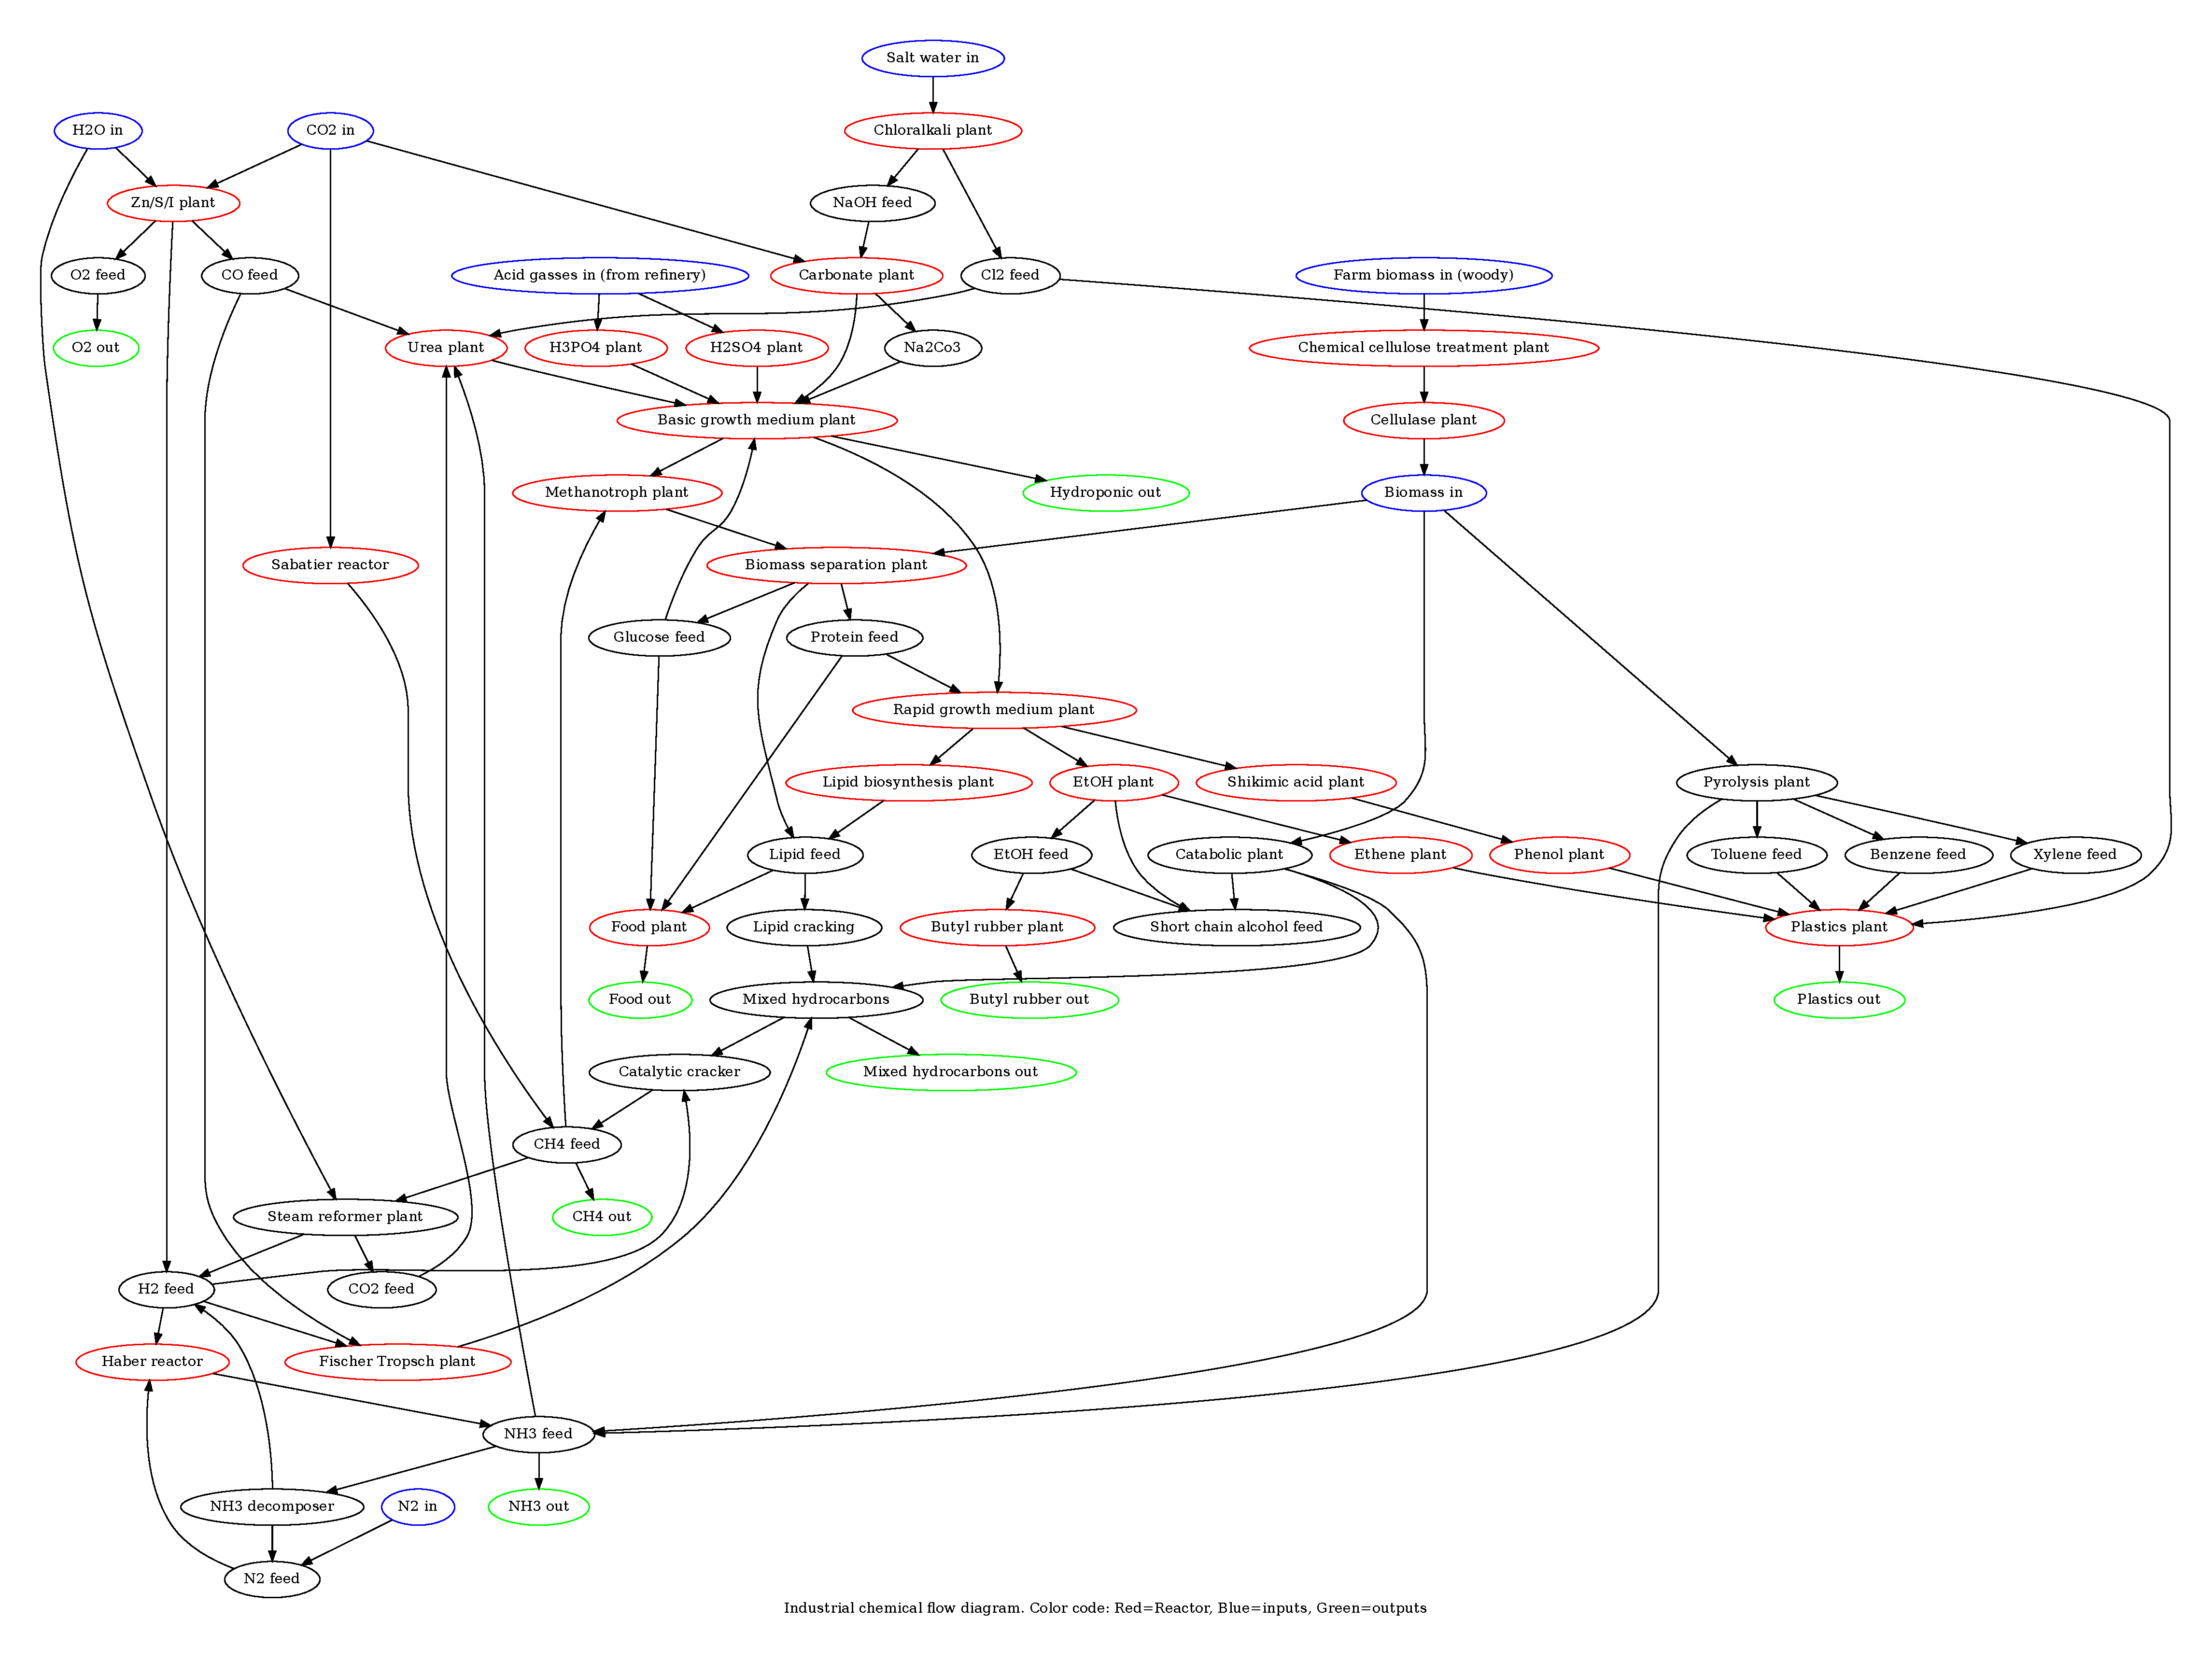
\includegraphics[width=\linewidth]{figures/fig_chem.pdf}
%    \caption{Chemical processing diagram}
%    \label{fig:chem_diagram}
%\end{figure}


% TODO: At the end of the overall section we could possibly play around with the wording here and reiterate the message we started with, which should seamlessly lead us into the next section. As mentioned previously, water is recycled through a two stage TSSE process, with air being produced through a multitude of pathways depending on market conditions. This market mechanism, along with having multiple pathways for production, then allows for a more robust production process. Similarly, by financially structuring the chemical commodities market through a common futures and spot market, capital for the expansion of production facilities can be easily obtained.


%---------------------------------------------------------------------------------
%	SECTION 2: LIFE ON MARS: SOCIETY AND ECONOMY
%---------------------------------------------------------------------------------

\section{Life on Mars: Society and Economy}
Having outlined the technical processes needed to sustain human life on Mars in \ref{sec:technical-design}, in this section, we lay out the defining characteristics of KCSAR's social and economic makeup. Throughout, we integrate commentary on the ways in which KCSAR's political, cultural and aesthetic makeup contribute to its vibrant society.

\subsection{Governance}
The KCSAR political system embodies the most direct feasible form of democracy, a delegative democracy. It has been argued that one of the greatest benefits of a direct democracy, is that it acts as a constraint on the actions of political elites, forcing them to represent the interests of the populace at large and to adopt cooperative rather than confrontational strategies \cite{Papadopoulos2001}. In practice, the direct democracy of KCSAR is governed by four distinct branches, with government powers separated between the executive, legislative, judicial, and an auditor branch.

Procedural laws substantially limit the powers of each of the branches of government, enforcing substantial oversight from each branch upon the others and requiring that for any substantial change in policy or exercise of non-standard powers, the issue is put to a ranked choice vote by all citizens. Additionally, where matters of judicial interpretation or issues raised by citizens receive a sufficient amount of public support, they are put to a vote. Thereby, citizens directly determine government decisions.

% Does this provide enough value to justify the space it's taking up? It seems rather large. 
    % I suggest we kill it, please reject my change if you disagree.
% Yeah, these diagrams are too large, let's see if we can get more useful stuff in instead

These democratic arrangements are unpopular on Earth primarily because of the prohibitive time cost associated with voting on such a broad range of issues. In KCSAR, this cost is limited through a system of vote delegation by which citizens may delegate their voting right to other individuals or between individuals based on the subject area of the vote. For example, a citizen may delegate their military decisions to person X and economic decisions to person Y. These delegations may be changed at any time and are supported using cryptographic primitives such as homomorphic encryption and linkable ring signatures, allowing for both anonymous voting and cryptographic security \cite{Kaye}.

To incentivize the emergence of delegates and enable them to publicize their voting positions, the government provides a stipend proportionate to the number of votes a delegate receives. Strict campaign financing laws prevent the use of external funds or exercising undue influence to promote a viewpoint. To ensure that decisions are data and logic-led and that a full range of opinions voting options are represented, 'index voters' - robot delegates that vote on specific issues which follow simple 'if then' logical statements or rely on more advanced techniques from machine learning - are employed. The data and logic used in their decision-making is open to the public and auditable.

\subsection{The Malthusian Trap}
The Malthusian Trap emerges where the average individual within an economy produces only as much as they require to live over their life cycle. Modern credit systems reframe the traditional problem by offering emerging economies the ability to finance the 'importation' of a high total factor productivity by utilising capital-intensive productive technologies. The viability the KCSAR economy thus turns on its ability to sustain a high enough economic output to exceed the combined costs of its existing debt burden (interest and loan repayments) and the costs of supporting its citizens. Hence, maintaining a high GDP per capita is the primary concern of KCSAR's emerging economy and its social design prioritises the maximization of GDP per capita, while supporting a more equitable distribution of resources than that found on Earth. Relatively equitable distribution of resources is important not only in ensuring that all citizens are provided for and live a life a without poverty, helping to enhance social stability, but also in generating higher domestic demand and therefore enabling higher productivity gains through economies of scale. \cite{Kogel} 

\subsection{Immigration}
Having highly productive citizens is a key priority of KCSAR. High demand to be part of Earth's first extra-planetary colony provided the opportunity to select for ideal candidates using an AI-based actuarial model of a citizen's lifetime production. However, the cost of travelling to KCSAR (USD 500k approx.) continues to make it difficult for otherwise ideal candidates, who are young, well-educated and therefore have limited wealth, to immigrate. The government subsidizes or underwrites a portion of these individuals' ticket prices, enabling them to access commercial loans by reducing the risk to banks of their default. Friends and families of family members are also encouraged to pool collateral to further reduce the risk associated with commercial loans. Thus, government interventions provide the opportunity for Earth's 'best and brightest' to join KCSAR.

\subsection{Fertility}
In the presence of extremely high immigration costs, for an isolated colony to maintain its population, the fertility rate must remain above the replacement rate (approx. 2.1 children per person capable of bearing children). In most developed nations, the fertility rate has been rapidly declining and the direct importation of the culture surrounding fertility in those nations to KCSAR would result in demographic collapse. The incentivization of child-rearing is therefore a first order concern.

In KCSAR, direct economic incentives, such as a Universal Basic Income ('UBI') are offered to guardians proportional to the number of children for which they care and these have been shown to improve fertility outcomes \cite{Kalwij, Bjorklund}. Non-cash incentives such as additional leave and guardian allowances are also offered. These incentives are routinely adjusted to maintain a stable fertility rate and help contribute to a culture that celebrates caring for large families while continuing to productively contribute to KCSAR society 
        
As the cost of raising children is substantial in both direct costs (such as providing food and atmosphere for the child) and indirect costs (such as the loss of productive labor of parents) KCSAR is concerned with the 'quality' of children - their capacity to contribute to GDP - as well as their quantity. 'Embryonic selection' is used to select for the most fit potential children. Gametes are extracted from parents and fused to form blastocysts \cite{Shulman}. A cell is taken from each blastocyst and its genome is fully sequenced using a nanopore sequencer. The full genome sequence is then processed to generate a polymorphism map that is analysed using artificial intelligence to determine a ‘fitness’ index score. To estimate this fitness function requires the search space be both explored and exploited simultaneously, posing a 'one-armed bandit' problem. Therefore, we use a regret minimising strategy to estimate the value to both individuals and society of particular phenotypes.

The KCSAR also faces a phenotypic diversity bottleneck created by the small size of its population. Studies have shown that a lower limit on a genetic bottleneck is in the tens of thousands, with higher estimates for K selective species like humans that have few offspring but vast resources available for them. As the population must thrive while adapting to the Martian environment, genetic diversity must be thought of as a resource with risk amelioration benefits even for a population as high as one million. Therefore, frozen gametes from screened and compensated individuals are imported to the KCSAR en masse. The transport costs are relatively low due to the light weight of the cargo.

\subsection{Demographics}
To project KCSAR's population demographics, we scale demographics from Gambia, which has a similar fertility rate (3.5 children/woman) and population growth rate (40\%). \cite{Gambia} In \ref{fig:demog_total} we approximate a demographic pyramid for KCSAR.

\begin{figure}
    \centering
    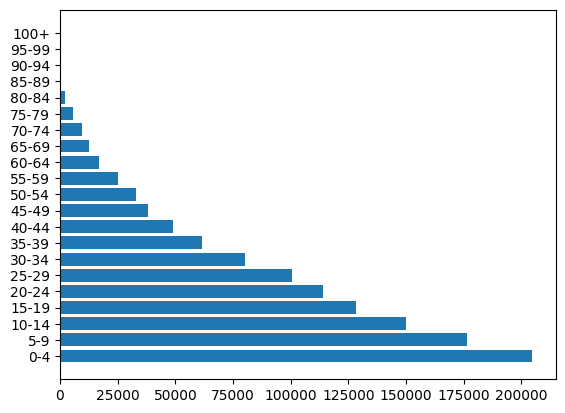
\includegraphics[width=85mm]{figures/fig_demopyr_t.png}
    \caption{Implied demographic pyramid}
    \label{fig:demog_total}
\end{figure}

Young children and the elderly are not part of the labor force and are provided for by the government. As the cost of providing for non-productive individuals is much higher on Mars than Earth, the proportion of people who are part of the working population must be relatively high. Assuming various cutoffs for the working age population, we project the occupations of citizens in \ref{fig:workingage}.

\begin{figure*}[t!]
    \begin{subfigure}[t]{0.45\textwidth}
        \centering
        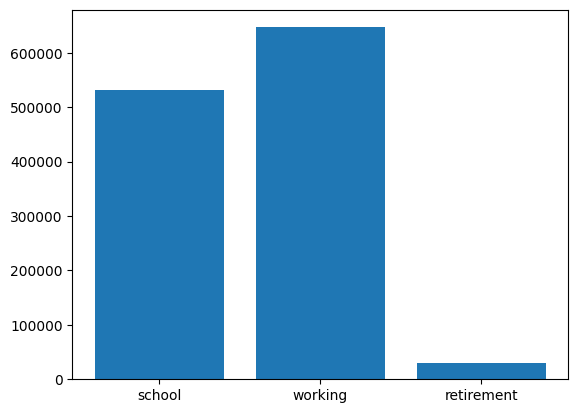
\includegraphics[height=55mm]{fig_demo_down.png}
        \caption{Workforce aged 15-64}
    \end{subfigure}
    \qquad \qquad  %This adds space between images
    \begin{subfigure}[t]{0.45\textwidth}
        \centering
        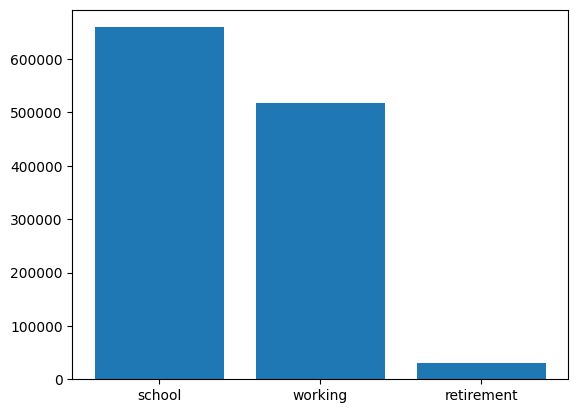
\includegraphics[height=55mm]{fig_demo.png}
        \caption{Workforce aged 20-64}
    \end{subfigure}%
\caption{Impact of working age cutoff on size of labour force}
\label{fig:workingage}
\end{figure*}

As is evident from \ref{fig:workingage}, the age at which young people enter the workforce has a dramatic impact on the ratio of working age people to others in a society with such a high reproductive rate. While the proportion of the population entering retirement is low, children engaged in schooling are a substantial burden on KCSAR. 

\subsection{Education}
Optimising the educational process and limiting the amount of time spent in education is one of the key methods to increase the size of the working population. With the advent of the information age, ever more efficient educational methodologies have emerged. KSCAR's educational facilities rely on developments in AI-assisted learning such as in optimising curriculum to the needs and abilities of individual students and in adapting examination difficulty to the level of students. Students are grouped together by ability, rather than age group and provided access to pre-recorded lectures, teaching assistants and learning materials from a variety of sources, enabling them to take ownership of maximising the speed of their learning experience. Curricula are simplified and specified to the greatest extent possible so that students are prepared to enter an occupation that reflects both their preferences and ability. Particularly for children, methods that focalize ‘learning through playing’ and student enjoyment are preferred to foster a culture that values and enjoys the process of learning and work.

\subsection{Work}
The majority of the workforce are engaged in key sectors laid out in KCSAR's technical design and the largest proportion are engaged as factory workers. KCSAR does not receive natural sunlight, so rather than relying on traditional day-night shift working cycles, KCSAR workers work to an eight-hour shift cycle that enables continuous work. To maximise the working population proportion, full employment is sustained through a federal jobs guarantee. All able-bodied workers are provided work at below market wages, enabling otherwise unemployed labor for government operations and ventures. Workers are also encouraged to engage in education to reskill to meet the needs of a dynamic labor marke and are provided significant subsidies.   

\subsection{Retirement}
KCSAR follows the Singaporean model for retirement saving. Each employee pays 10\% of their gross income to purchase stock of the KCSAR Sovereign Wealth Fund (‘KCWF’). The KCWF is a trust, managed by the government, which invests in the equity and debt of local businesses. The value of the KCWF grows at the roughly average rate of the market on KCSAR. On retirement, workers sell down their units to fund a pension. For most workers, this is a sufficient pension but the government contributes to pensions that do not meet a specified living wage cutoff. The sovereign wealth fund receives proceeds from the sale of land, mineral rights, patents generated by public universities and other public goods.

\subsection{System of wages}
All KC citizens receive a Universal Basic Income (‘UBI’), which is a cash payment indexed to the cost of a basket of essential goods and services. The provision of a UBI produces a society in which the basic needs of all citizens are met, which has four primary benefits: 

\begin{enumerate}
    \item On Mars, where space and air have material costs, unemployment and homelessness have even larger social burdens. A UBI provides a security net, helping to tide people over and thereby reducing the number of people who are initially part of cyclical or frictional unemployment from becoming long-term unemployed.
    \item Studies have shown that there is a strong association between relative poverty and crime. In a Mars colony, where crime is relatively difficult and expensive to prosecute, making sure that all individuals have access to a living wage may be a cost-saving measure \cite{Hooghe}.
    \item It provides support to unpaid care workers and individuals who are not engaged in the formal workforce. This in turn relieves pressure on public services that provide care to ill and differently abled people as well as incentivizing the growth of families.  
    \item It simplifies the provision of transfer payments to citizens by eliminating the need for secondary transfer payments. 
\end{enumerate}

The primary objections to a UBI are that it reduces motivation to work and that it perpetuates inequity, as the most wealthy individuals receive the same benefit as the poorest. Incentives to work still exist with a UBI as the receipt of a wage above the UBI award rate is associated with far greater access to luxury goods and particularly preferred foods such as fish and meat. Moreover, a UBI eliminates the structure of adverse incentives that may arise from other social security programs. Traditional social security programs may offer negative net wages for marginal increases in hours worked, whereas the return from work strictly exceeds the additional taxation burden under a UBI system. In KCSAR, the UBI also has a positive net impact on the equitable distribution of income as it is accompanied by a progressive taxation system such that for anyone of middle class or above, the total value of tax paid exceeds the value of the UBI. 

While there is no economy-wide, government mandated ‘minimum wage’ in the KCSAR, unions are formed within each major industry that then demand appropriate working conditions and remuneration for members. In guaranteeing that the returns of corporations are distributed to labor (rather than absorbed entirely by capitalists), labor unions serve an important role in allocating resources to the population most likely to spend them and encourage further growth, as the Marginal Propensity to Consume (‘MPC’) of workers is higher than that of wealthier business owners. These labor unions will operate as delegative institutions. As companies grow larger, the importance of their unions also grows and unions will take on a direct oversight role as members of the company board. 

\subsection{Taxation}
The taxation mix broadly aims to incentivize taxpayers to engage in the most efficient economic activities (maximising GDP per capita) whilst remaining progressive (maintaining a minimum degree of inequitability). The largest component of the taxation mix is a simple income tax, that is highly progressive and ensures that the net effect of the UBI is positive for low income earners but negative for higher ones. Additionally, a substantial inheritance tax will be utilised to reduce wealth inequality and encourage social mobility. Lower wealth inequality is associated with higher capital mobility, as wealth is negatively correlated with MPC and higher social mobility likely improves labor engagement and provides incentives for hard work and innovation \cite{Brueckner-2018}.

Taxation is also used as a lever to encourage productive economic behaviors. Capital gains taxes are levied on the increased value of capital goods with active asset rollover exemptions that allow for deferral or reduction of tax burden if the profits generated from the sale of a capital asset are reinvested in new capital assets. This will creates an incentive for individuals to reinvest returns, helping to improve liquidity in the capital market and grow the economy as a whole. Land value taxes are levied on the unimproved value of the real estate of the colony (on shops, apartments etc.). This creates an incentive for land to be used for its most efficient purpose and thereby encourages the endogenous formation of regional specialisation. For example, if an area of land were an industrial zone, and it would be more productive for that land to be used for the creation of a shopping area, the tax provides an economic incentive for the industrial zone to relocate, likely to areas that already have a mass of industrial sites, where firms can benefit from the economies of scale of regional specialisation.

\subsection{Property Market}
Within the city of KCSAR, land is granted to private individuals for a fixed duration and may be traded, mortgaged and rented. As each new section of the city is built, the ‘land’ inside is sectioned off for land deeds with a fixed ownership term, which is its design refurbishment lifetime (around 30 to 50 years into the future). On the expiry of the grant, the land is returned to the government, refurbished, redivided and reallocated. This model leads to land growing cheaper over time, making it more accessible to first home buyers. Additionally, mortgages are easily bundled together into collateralized mortgage obligations and are traded between banks, providing a substantial source of liquidity for the short term loan market.

\subsection{Regulation of natural monopolies}
Many of KCSAR's essential markets are natural monopolies in which the cost function of mass production is more highly correlated with the number of distinct designs produced, rather than the number of items that each produces. In particular, regulated modules are the building blocks of the multitude of designs required to service the colony's needs. As these must be produced at scale, through an Original Design Manufacturing model, to minimise costs, they form a natural monopoly. To make these monopolistic industries profitable, while limiting the undue usage of monopoly power, a regulated utility corporation model is used. Candidate organisations are offered monopolitic control over a sector as well as cheap loans provided through the KCWF in exchange for significant public oversight. The charters offered to these organisations issue board seats that are mangaged by the community through delegative democracy. The audit branch is given additional powers to inspect company documents, ensure compliance and to provide the public a means of redress. This oversight also ensures that these corporations are extremely stable, making them ideal candidates for conservative investors.

\subsection{Law and order}
On Mars, the cost of incarceration is prohibitive, as the cost of space and providing for individual citizens are extremely high. KCSAR implements a rehabilitative rather than retributive model of justice that aims to limit the incentives for crime and to prevent the emergence of environments that may encourage radicalisation. It prioritises early intervention programs that identify and satisfy the needs of citizens experiencing hardship. The political and economic system outlined above also ensures that every individual has a say in government decision-making as well as access to meaningful work and the promise of a bright future. This removes some of the key incentives around which larger scale structural crime might develop \cite{10.1093/bjc/azq067}. Policies and monitoring are also implemented to prevent ghettoization, and thereby structural disprivilege that may lead to structural crime. 

\subsection{Leased rockets}
An increasingly mature market for leased rockets is pivotal in the reduction of costs associated with interplanetary travel and for the viability of interplanetary trade. A leasing market for reusable rockets enables relatively small companies involved in interplanetary travel and commerce to operate despite extremely high startup costs. As rockets are extremely expensive purchases and proper actuarial models to determine the risk associated with the asset did not yet exist, an insurance policy for the potential shortfall was created to ensure the profitability of investing in rocket ownership. The insurance policy relied on the usage of catastrophe bonds and government intervention through targeted reinsurance programs that restrict the unhedged risk to the insurer to standard commercial risks. This enabled the repackaging and reselling of debt with the same credit rating as the insurer and thereby the on-selling of leases on the wholesale debt market, refilling the initial fund and including extra profit on the lease (a Credit Default Swap). As the market continues to mature and the asset risk is better understood, liquidity continues to improve.

\subsection{Significance and composition of trade}
As an isolated colony, KCSAR remains dependent on key imports from Earth including pharmaceuticals; chemical reagents that are prohibitively expensive or impossible to produce on mars; silicon; and other consumer and capital goods. As the cost of transport is prohibitively high at \$500/kg, these goods are imported in their most weight efficient form. For example, bulk pharmaceuticals are transported as active ingredients and undergo final transformation on Mars. To incentivize importation of capital goods to improve firm productivity, the KCWF is also used to subsidise the import of capital goods. 

To purchase these crucial imports, KCSAR must produce a sufficient quantity of exports. The prohibitive costs of transporting goods to Earth (\$200/kg) requires that only products with extremely high value-add to weight ratios be exported. These products include:

\begin{enumerate}
\item Precious materials are mined from asteroids near Mars by 'Honeybee-style' automated robotic mining. Modelling of the price elasticity of demand for gold, platinum and other precious metals indicates that significant quantities may be exported before oversaturation of supply makes it uneconomical. The movement of mined goods and intra-colony trade is facilitated by 'nuclear hoppers' - relatively cheap reusable single stage nuclear thermal rockets that use martian CO2 as propellant \cite{Zubrin2011}.
\item Fuel mined from comets is exported to refueling stations around the solar system. These stations enable spacecraft that would only able to reach Low Earth Orbit to reach Mars and the outer solar system via an on orbit refueling stage.
\item Creative and productive intellectual property produced on Mars serves as a key export. In particular, on Mars, there is a greater imperative to semi-automate or completely automate tasks, producing a comparative advantage in the creation of some AI systems, designs and datasets. Where applications for efficiency gains in Earth-bound processes are found, these assets are exported with close to zero marginal cost.
\item  The sale of debt and equity will also serve as a key ‘export’ that will finance ventures on Mars, helping to stabilize the balance of trade. In particular capital intensive projects such as mining ventures and infrastructure projects will require external financing which will be recorded as a credit on the capital account.
\item Mars will also has a competitive advantage in the building and operation of telescopes, probes and landers that are to be launched to the far reaches of the solar system. For example, the building of large scale mirrors is far easier on Mars due to its low gravity and access to a vacuum. Some peaks on Mars, such as Olympus Mons also serve as a good location for deep field astronomy.
\item Mars is an ideal candidate for large scale nuclear production, so isotropic extraction from spent fuel will be a significant source of revenue. Nuclear isotopes such as Pu240, Am241 and Co60 are extremely expensive on Earth but would be relatively easy to produce on Mars. Pu240 is used in space probes that are likely to be built nearby in any case.
\item In the future, it’s likely that more uses for zero and low gravity as well as vacuum environments will emerge. It is already clear that some types of research are only possible in these environments. Leasing out space in KC and providing labor to conduct experiment and create these goods may therefore constitute a substantial source of revenue. 
\end{enumerate}

\subsection{The mechanics of trade}
The exchange of packages through the inter-planetary postal services is the basis for trade between KCSAR and earth-bound parties. The KCSAR is a member of the United Postal Union (UPU) and therefore part of the standard postal infrastructure between member states. The distribution network relies on ‘multi-modal’ routing, by which packages are carried by the most cost (or time, depending on the cargo) efficient mixture of trucks, trains, boats, and planes. "Cargo is transported in standardized containers, allowing for the economies of scale created through standardized packing and handling that have been realised on earth to dramatically reduce the cost of transporting goods to mars." \cite{Levinson}

As Mars is crucially reliant on imports of some necessities, the economic viability of the transportation system that underpins trade is a primary concern. The key results of a sensitivity analysis, shown in \ref{fig:reuse}, \ref{fig:numflights}, \ref{fig:flight_cost_cap} and \ref{fig:flight_cost_launch}, indicate that the primary mechanism for reducing the transport cost for delivery of freight to Mars is increasing the lifespan and reusability of leased rockets (at least to the 10-year mark). We take the partial derivative of price with respect to a vector of potentially explanatory input variables to provide an indication of how much a change in each factor would impact price. While the rocket lifespan effect dominates, secondary factors such as reducing launch costs (by, for example, connecting the launch complex on Earth to a natural gas pipeline) and reducing the cost of rockets would have significant impact. The technological innovation and reduction in cost of factors of production necessary to change these key factors is most easily stimulated through economies of scale. To enable these economies of scale, a significant market must be generated to enable producers to benefit from scaling up production facilities and investing in research and development.

%This one is important as they show the main thesis here - that increasing lifetime and reusability provides large improvements to cost.
\begin{figure}
    \centering
    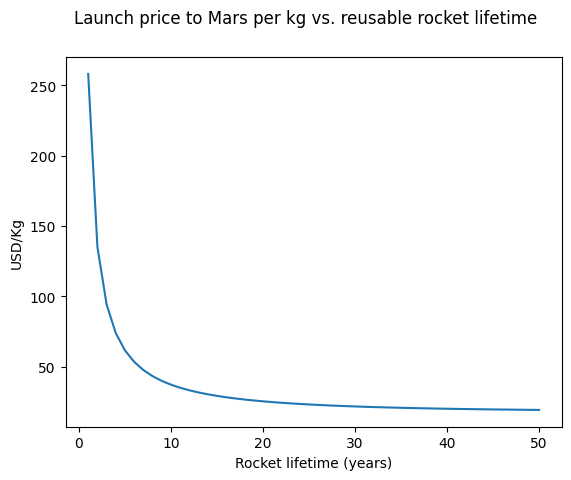
\includegraphics[width=\linewidth]{fig_reuse.png}
    \caption{Launch price to mars vs. reusable rocket lifetime}
    \label{fig:reuse}
\end{figure}

\begin{figure}
    \centering
    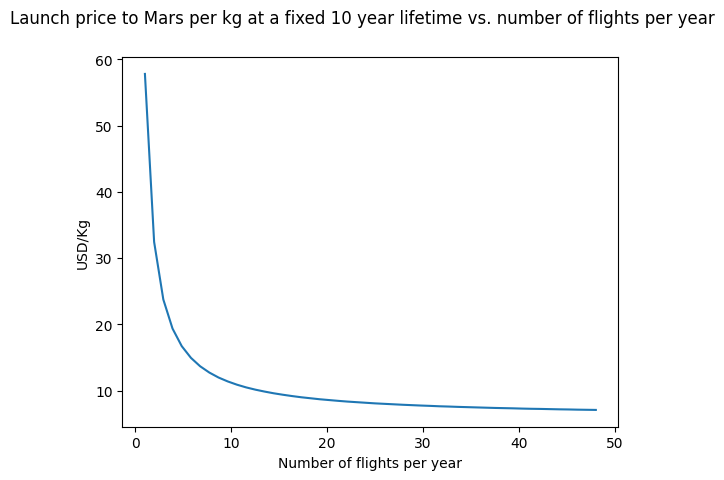
\includegraphics[width=\linewidth]{fig_numflights.png}
    \caption{Launch price to mars vs. number of flights per year at fixed 10 year lifetime}
    \label{fig:numflights}
\end{figure}

%These figure is less important and can be cut if we run out of space - it can be replaced with a sentence akin to 'As capital costs or launch costs decrease, launch price drops linearly'. There's a similar graph for per launch cost going down.

\begin{figure}
    \centering
    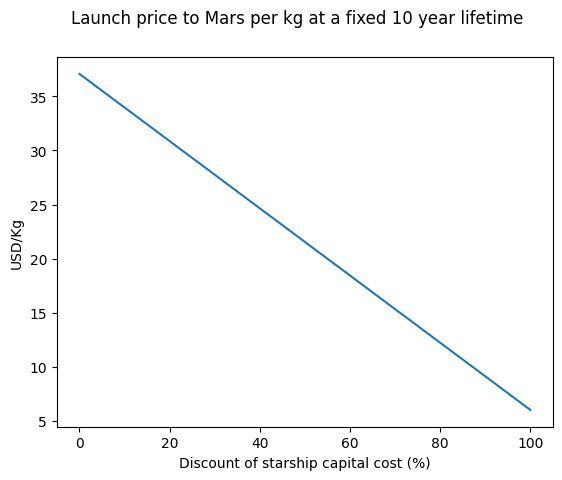
\includegraphics[width=\linewidth]{fig_discflights.png}
    \caption{Launch price to mars vs. discounted capital cost}
    \label{fig:flight_cost_cap}
\end{figure}

\begin{figure}
    \centering
    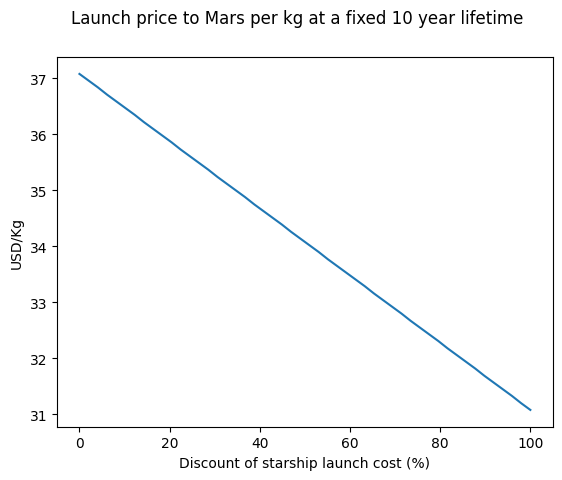
\includegraphics[width=\linewidth]{fig_disclaunchflights.png}
    \caption{Launch price to mars vs. discounted launch cost}
    \label{fig:flight_cost_launch}
\end{figure}

Three mechanisms are used to generate stable demand for interplanetary trade: government intervention in its futures market and competition regulation. A futures market for interplanetary trade emerged endogenously, helping to stabilize the demand for and price of traded goods and thereby enabling small and marginal producers to reduce their exposure to liquidity risk and enter the market. It also encouraged more efficient allocation of resources over time. The government intervened by providing a demand floor for interplanetary trade by consistently buying futures for freight transport and using them to transport mail, capital and other government materials. An independent watchdog monitors, reports and provides recommendations to the government on non-competitive behaviors in the rocket production industry. Due to the substantial start-up costs and competitive advantage associated with holding intellectual property in the industry for producing and maintaining rockets. The emergence of vertically integrated firms and firms with substantial market (monopolistic) power is therefore likely. Through the use of the leased rocket model, nonintegrated rocket production companies can easily support an ecosystem of launch providers if they are encouraged to through substantive oversight. A substantially competitive market will keep the costs of production low and encourage innovation amongst competing firms.

\subsection{Culture}
Given that the residents of KCSAR face extraordinary labor and resource scarcity and live in closely contained quarters, it is critical its emerging culture is one that: (a) cultivates a passion for work that is motivated by a desire to advance the collective interests of the colony, (b) values close communal relationships, (c) fosters and applauds innovative thinking, (d) promotes an appreciation and love for both knowledge acquisition, and knowledge sharing, through a life-long pursuit of education, and (e) celebrates large families. To develop these cultural tenets, many of the societal superstructures (e.g. the design of shared spaces, immigration selection criteria, human resource allocation, food manufacturing, among others), are implemented in a way that aligns with and encourages this cultural ethos.

Perhaps the most powerful example of such cultural 'nudges' is in the aesthetic and architectural design of KCSAR's city. A government regulation mandates that all domes contain a government-subsidised cultural center at its focal point.The cultural center is made up of three concentric circles defined by an open plan aesthetic that encourages social engagement. In the innermost circle exists a place where community members are provided with free access to the internet, luxurious recreational seating, local food delicacies, and encouraged to engage prize-giving activities that foster intellectual expression, such as debates and hackathons. To reach the innermost circle, community members make their way across the two outermost circles, which are designed to share and celebrate local achievements. For example, local artists and hospitality workers are encouraged to express themselves in the outermost circle, with public displays of original music, food, and art and government grants are available for the creation of such works. In the middle circle, virtual presentations adorn the walls, showcasing the accomplishments of local scientists, innovators, and business champions. In this way, a cultural ethos that simultaneously perpetuates artistic expression, intellectual inquiry, originality, innovation, and collaboration is encouraged. 

The government also takes a more direct role by providing economic incentives for individuals to engage in childrearing and education, as detailed previously, as well as providing educational campaigns (for example, tv infotainment campaigns) that encourage socially beneficial behaviours. For example, as living and working in the difficult close contact conditions of a Mars colony has ramifications for people's mental health and life satisfaction, these programs encourage people to form tight-nit relationships with their close neighbours and provide information about how to form supportive relationships that improve mental health outcomes. Self expression through the arts and recreational activities are also highly encouraged and subsidised through government grants.

\subsection{The future of KCSAR}
To this point, we have laid out the bare bones social and economic processes needed to support a colony of one million people facing pressing existential risk. We turn now, by way of conclusion, to look at what the future will hold. 

Over the coming years, a substantial geoscaping operation will be implemented to make the Crater habitable for humans. A central aluminium space frame-style construction with a series of support pillars will hold up a cover, consisting of a thin PHB or other bioplastic layer and a clear layer of lipid-derived wax, acting as a counterweight to the air pressure beneath and thermal insulation. This greenhouse structure will be filled with the potent greenhouse gas, SF6, until it reaches the Armstrong limit, increasing the Crater temperature to above 0\degree{}C. The Crater’s ice layer will melt, forming a glacial lake. Evaporation of water vapour from the lake can then occur, improving the atmospheric pressure within the Crater. O2 and Ar will then be pumped into the atmosphere to make it habitable for human and other air-breathing life.

The lake will be seeded with nutrients, including metal trace nutrients, sulfates and phosphates to make it habitable for plants and algae. Azolla and algae will be added to produce food and oxygen, whilst fixing nitrogen from the atmosphere. Once it is habitable, the lake will be seeded with fish that will become an important food source for the KCSAR colonists. The upper barrier will form artificial rain clouds as it cools warm moist air that condenses into water and falls as rain. Animals will be able to walk freely about the surface and the lake will be green with life. 

\begin{figure}
    \centering
    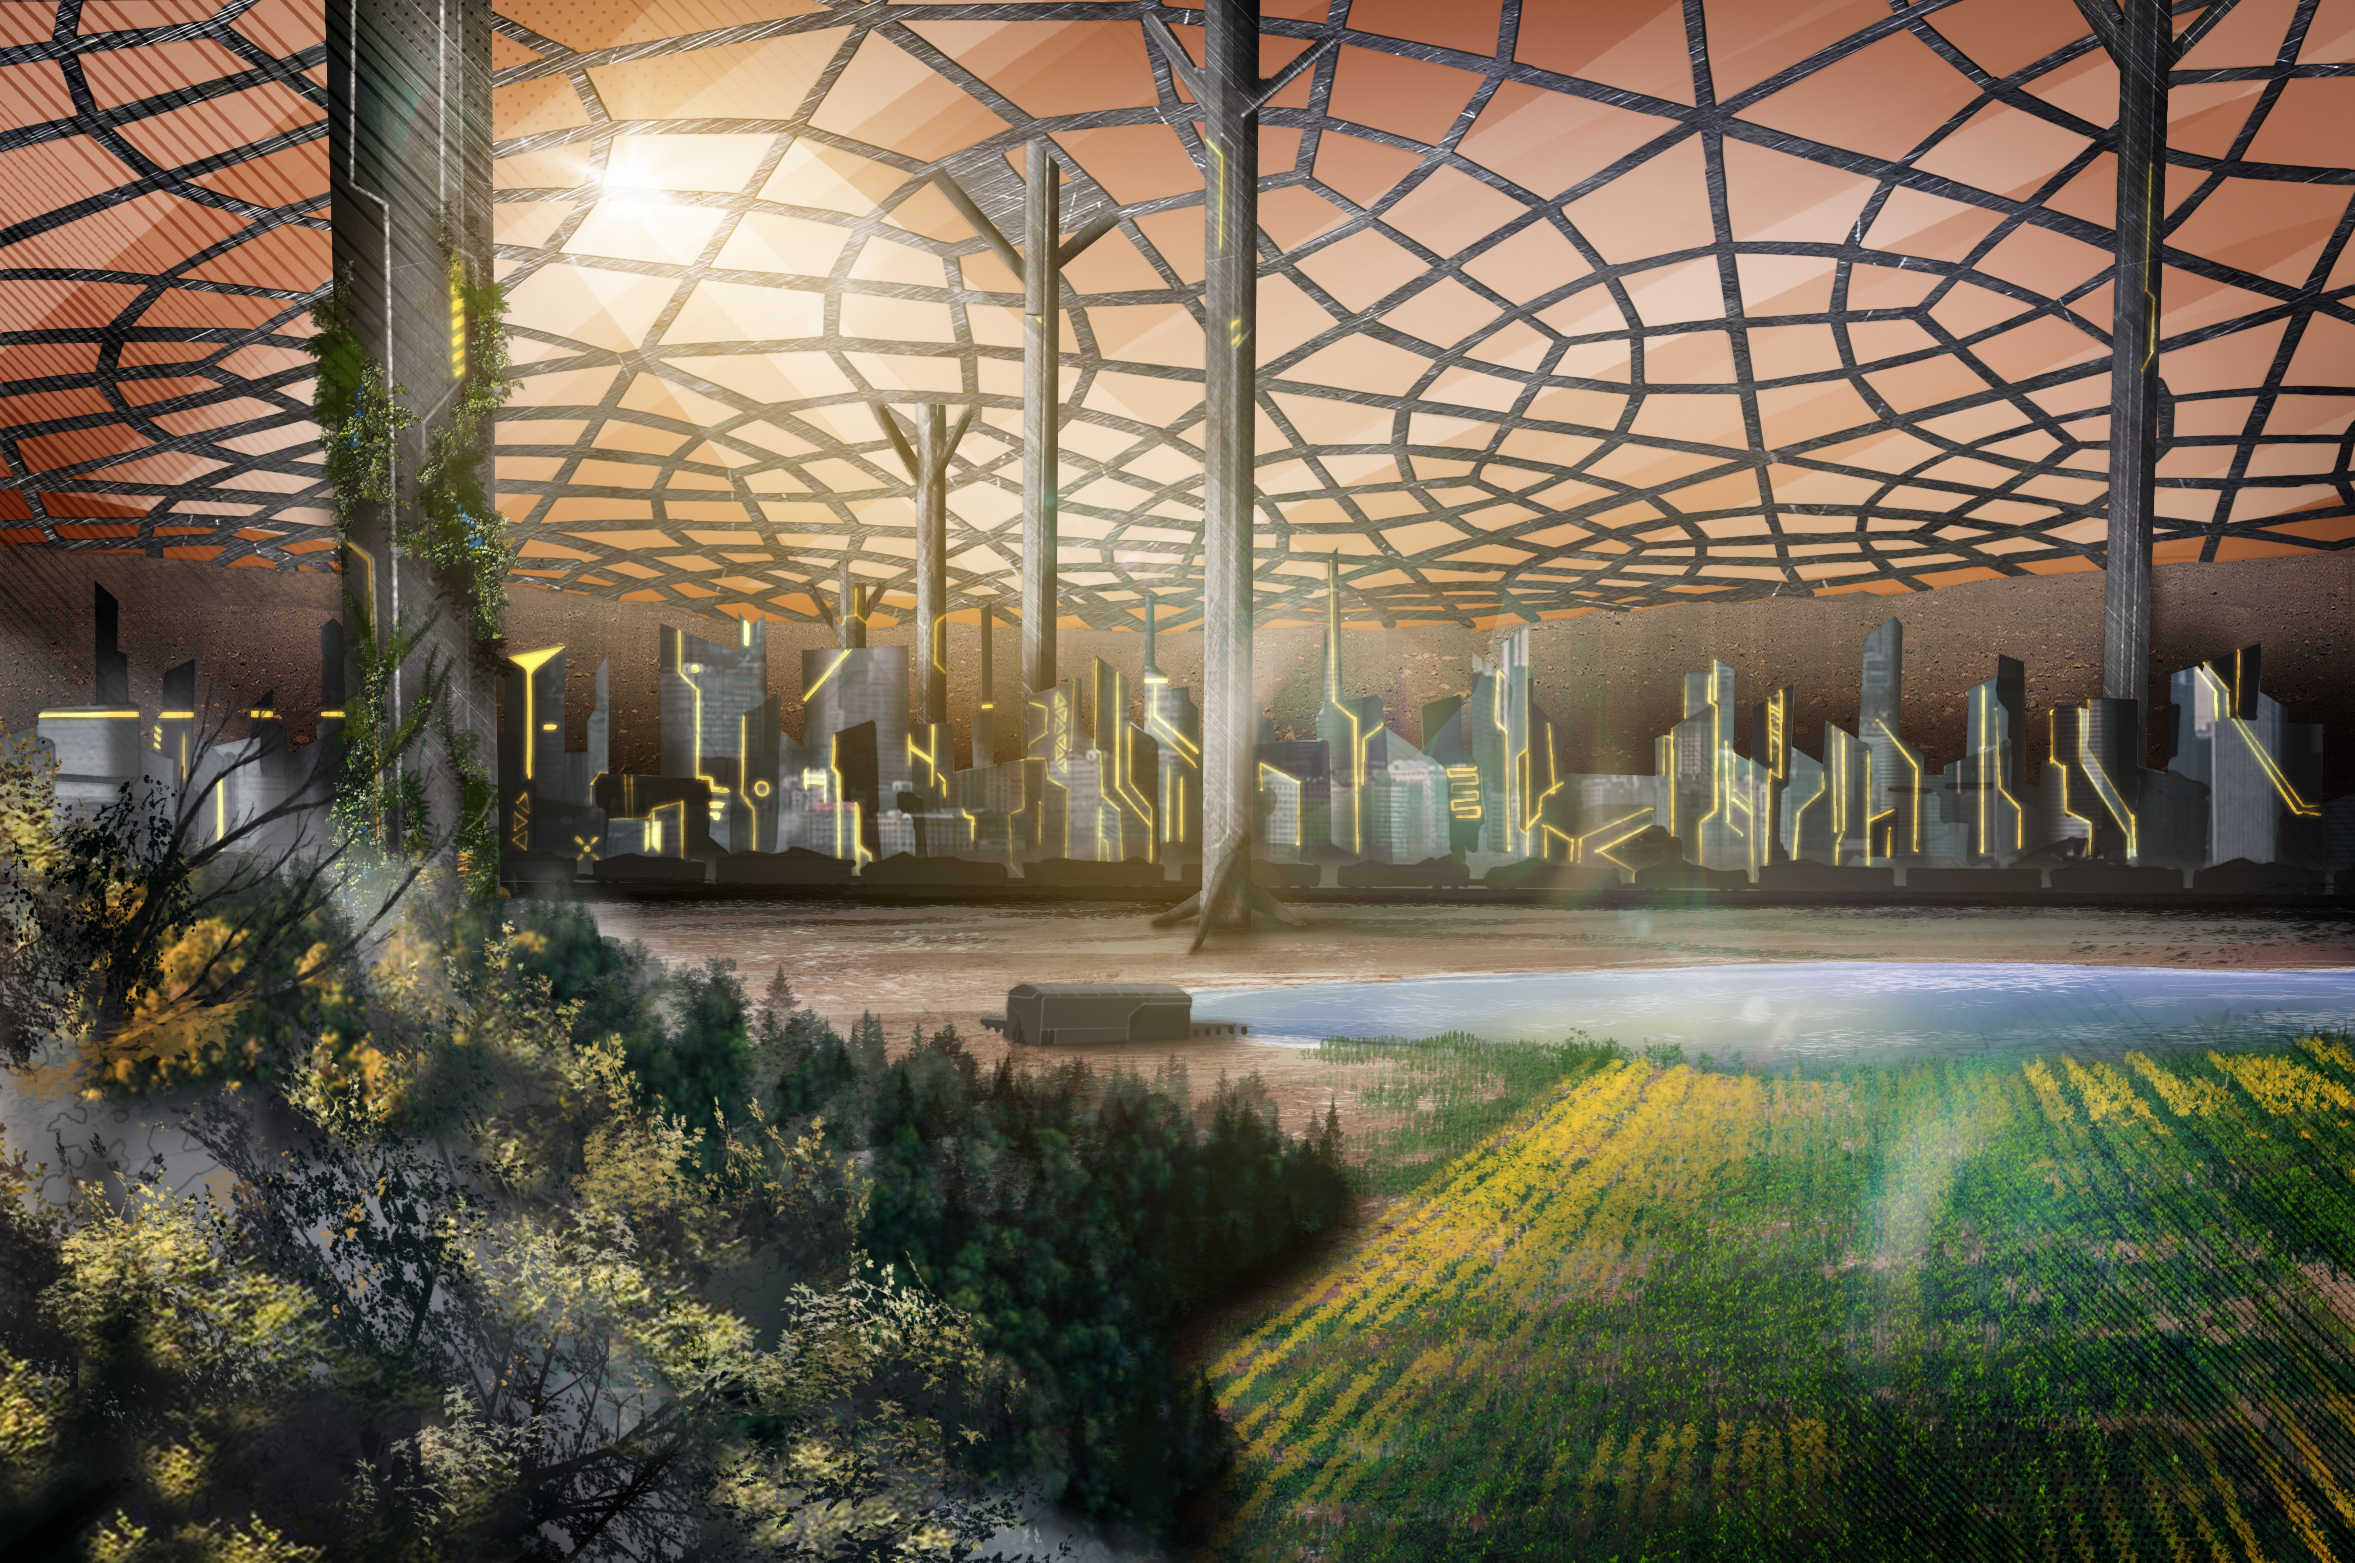
\includegraphics[width=\linewidth]{art/terraformed_dome.jpg}
    \caption{Artist's rendition the future terraformed crater}
    \label{fig:final_dome}
\end{figure}

%---------------------------------------------------------------------------------
%	SECTION 3: ACKNOWLEDGEMENTS:
%---------------------------------------------------------------------------------
% \phantomsection
\section*{Acknowledgments} % The \section*{} command stops section numbering
\addcontentsline{toc}{section}{Acknowledgments} % Add to Table of Contents

Alex please fill in acknowledgements here 
%---------------------------------------------------------------------------------
%	SECTION 4: BIBLIOGRAPHY
%---------------------------------------------------------------------------------
\phantomsection
\bibliographystyle{unsrt}
\bibliography{references}

%---------------------------------------------------------------------------------
%   END DOCUMENT
%---------------------------------------------------------------------------------
\end{document}